\chapter{Elements of Point Set Topology}

\section{Open and Closed Sets in $\mathbb{R}^1$ and $\mathbb{R}^2$}

\subsection*{Definitions and Theorems for Section 3.1}

\begin{definition}[Open Set]
A set $S$ in a metric space $(M,d)$ is said to be open if for every point $x \in S$, there exists a positive number $\varepsilon$ such that the open ball $B(x;\varepsilon) = \{y \in M : d(x,y) < \varepsilon\}$ is entirely contained in $S$.
\end{definition}

\noindent\textbf{Importance:} Open sets are the fundamental building blocks of topology. They formalize the intuitive notion of "neighborhoods" and provide the foundation for understanding continuity, convergence, and many other topological concepts. Open sets are essential for all areas of analysis, topology, and modern mathematics.



\begin{definition}[Closed Set]
A set $S$ in a metric space $(M,d)$ is said to be closed if its complement $M \setminus S$ is an open set.
\end{definition}

\noindent\textbf{Importance:} Closed sets are the dual concept to open sets and are equally fundamental in topology. They capture the idea of sets that contain all their limit points and are essential for understanding compactness, completeness, and many other important topological properties. Closed sets are crucial for analysis and many applications in mathematics.



\begin{definition}[Interior Point]
A point $x$ in a metric space $(M,d)$ is said to be an interior point of a set $S \subseteq M$ if there exists a positive number $\varepsilon$ such that the open ball $B(x;\varepsilon)$ is entirely contained in $S$.
\end{definition}

\noindent\textbf{Importance:} Interior points formalize the intuitive notion of points that are "inside" a set, not on the boundary. They are essential for understanding the structure of sets and are crucial for defining the interior of a set. Interior points are fundamental for topology and many areas of analysis.



\begin{definition}[Accumulation Point]
A point $x$ in a metric space $(M,d)$ is said to be an accumulation point (or limit point) of a set $S \subseteq M$ if every open ball centered at $x$ contains at least one point of $S$ different from $x$ itself.
\end{definition}

\noindent\textbf{Importance:} Accumulation points are fundamental for understanding the structure of sets and convergence. They capture the idea of points that can be approached by sequences in the set and are essential for defining closed sets, compactness, and many other important topological concepts. Accumulation points are crucial for analysis and topology.



\begin{definition}[Neighborhood]
A neighborhood of a point $x$ in a metric space $(M,d)$ is any open set that contains $x$.
\end{definition}

\noindent\textbf{Importance:} Neighborhoods formalize the intuitive notion of "nearness" and provide a way to talk about local properties of spaces and functions. They are essential for understanding continuity, convergence, and many other topological concepts. Neighborhoods are fundamental for topology and analysis.



\begin{theorem}[Basic Properties of Open and Closed Sets]
In any metric space $(M,d)$, the following properties hold:
\begin{enumerate}
\item The empty set $\emptyset$ and the whole space $M$ are both open and closed sets.
\item The union of any collection of open sets is an open set.
\item The intersection of any finite collection of open sets is an open set.
\item The intersection of any collection of closed sets is a closed set.
\item The union of any finite collection of closed sets is a closed set.
\end{enumerate}
\end{theorem}

\noindent\textbf{Importance:} These properties are the fundamental axioms that define a topology. They establish the basic rules for how open and closed sets behave under set operations and are essential for all of topology and analysis. These properties are used constantly in proofs and are the foundation for understanding topological spaces.



\begin{theorem}[Characterization of Connectedness]
A metric space $(M,d)$ is connected if and only if the only subsets of $M$ that are both open and closed are the empty set $\emptyset$ and the whole space $M$ itself.
\end{theorem}

\noindent\textbf{Importance:} This theorem provides a fundamental characterization of connectedness in terms of open and closed sets. It gives a practical way to test whether a space is connected and is essential for understanding the structure of topological spaces. Connectedness is crucial for many results in analysis, including the intermediate value theorem.



\begin{definition}[Dense Set]
A set $A$ in a metric space $(M,d)$ is said to be dense in $M$ if every point of $M$ is either in $A$ or is an accumulation point of $A$. Equivalently, $A$ is dense in $M$ if the closure of $A$ equals $M$, that is, $\overline{A} = M$.
\end{definition}

\noindent\textbf{Importance:} Dense sets are fundamental for understanding the structure of metric spaces and are essential for approximation theory. They provide a way to approximate any point in a space using points from a subset. Dense sets are crucial for many results in analysis, functional analysis, and approximation theory.



\begin{theorem}[Density of Rational and Irrational Numbers]
Both the set of rational numbers and the set of irrational numbers are dense in the real line $\mathbb{R}$.
\end{theorem}

\noindent\textbf{Importance:} This theorem shows that both rational and irrational numbers are densely distributed throughout the real number line. This property is fundamental for understanding the structure of the real numbers and is essential for many results in analysis, approximation theory, and number theory. It demonstrates the richness of the real number system.





\begin{problembox}[3.1: Open and Closed Intervals ]
\begin{problemstatement}
Prove that an open interval in $\mathbb{R}^1$ is an open set and that a closed interval is a closed set.
\end{problemstatement}
\end{problembox}

\noindent\textbf{Strategy:} Use the definition of open sets (every point is an interior point) and closed sets (complement is open). For open intervals, show that every point has a neighborhood contained in the interval. For closed intervals, show that the complement is open by finding neighborhoods for points outside the interval.

\bigskip\noindent\textbf{Solution:} Let $(a,b)$ be an open interval in $\mathbb{R}^1$. To show it's open, we need to prove that every point $x \in (a,b)$ is an interior point. For any $x \in (a,b)$, let $\varepsilon = \min\{x-a, b-x\}$. Then the open ball $B(x,\varepsilon) = (x-\varepsilon, x+\varepsilon)$ is contained entirely within $(a,b)$. This shows that every point in $(a,b)$ is an interior point, so $(a,b)$ is open.

For a closed interval $[a,b]$, we need to show its complement $\mathbb{R} \setminus [a,b] = (-\infty,a) \cup (b,\infty)$ is open. Any point $x$ in this complement is either less than $a$ or greater than $b$. If $x < a$, let $\varepsilon = a-x$, then $B(x,\varepsilon) = (x-\varepsilon, x+\varepsilon) \subset (-\infty,a)$. If $x > b$, let $\varepsilon = x-b$, then $B(x,\varepsilon) \subset (b,\infty)$. This shows the complement is open, so $[a,b]$ is closed.\qed


\begin{problembox}[3.2: Accumulation Points and Set Properties]
\begin{problemstatement}
Determine all the accumulation points of the following sets in $\mathbb{R}^1$ and decide whether the sets are open or closed (or neither).
\begin{enumerate}[label=\textbf{(\alph*)}]
\item All integers.
\item The interval $(a, b)$.
\item All numbers of the form $1/n$,\quad $(n = 1, 2, 3, \dots)$.
\item All rational numbers.
\item All numbers of the form $2^{-n} + 5^{-m}$,\quad $(m, n = 1, 2, \dots)$.
\item All numbers of the form $(-1)^n + (1/m)$,\quad $(m, n = 1, 2, \dots)$.
\item All numbers of the form $(1/n) + (1/m)$,\quad $(m, n = 1, 2, \dots)$.
\item All numbers of the form $(-1)^n / [1 + (1/n)]$,\quad $(n = 1, 2, \dots)$
.
\end{enumerate}
\end{problemstatement}
\end{problembox}

\noindent\textbf{Strategy:} For each set, identify accumulation points by finding points that can be approached by sequences in the set. For openness/closedness, check if every point is interior (open) and if the complement is open (closed). Use density properties of rationals and convergence of sequences.

% Visualization for Exercise 3.2: Accumulation Points
\begin{figure}[h]
\centering
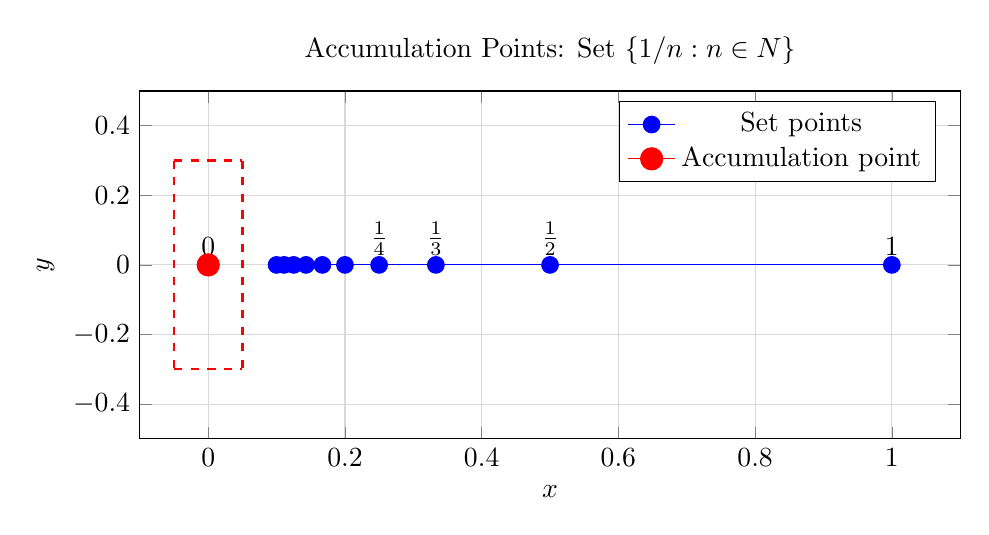
\begin{tikzpicture}
\begin{axis}[
    width=12cm,
    height=6cm,
    xlabel={$x$},
    ylabel={$y$},
    title={Accumulation Points: Set $\{1/n : n \in \mathbb{N}\}$},
    xmin=-0.1, xmax=1.1,
    ymin=-0.5, ymax=0.5,
    grid=major,
    grid style={gray!30},
    legend pos=north east
]

% Points of the set
\addplot[blue, mark=*, mark size=3pt] coordinates {
    (1,0) (0.5,0) (0.333,0) (0.25,0) (0.2,0) (0.167,0) (0.143,0) (0.125,0) (0.111,0) (0.1,0)
};
\addlegendentry{Set points}

% Accumulation point
\addplot[red, mark=*, mark size=4pt] coordinates {(0,0)};
\addlegendentry{Accumulation point}

% Neighborhood around accumulation point
\addplot[red, dashed, thick] coordinates {(-0.05,0.3) (0.05,0.3)};
\addplot[red, dashed, thick] coordinates {(-0.05,-0.3) (0.05,-0.3)};
\addplot[red, dashed, thick] coordinates {(-0.05,0.3) (-0.05,-0.3)};
\addplot[red, dashed, thick] coordinates {(0.05,0.3) (0.05,-0.3)};

% Labels
\node[above] at (axis cs:1,0) {$1$};
\node[above] at (axis cs:0.5,0) {$\frac{1}{2}$};
\node[above] at (axis cs:0.333,0) {$\frac{1}{3}$};
\node[above] at (axis cs:0.25,0) {$\frac{1}{4}$};
\node[above] at (axis cs:0,0) {$0$};

\end{axis}
\end{tikzpicture}
\caption{The set $\{1/n : n \in \mathbb{N}\}$ has 0 as its only accumulation point. Any neighborhood of 0 contains infinitely many points from the set.}
\end{figure}

\bigskip\noindent\textbf{Solution:} 
(a) The set of integers has no accumulation points since each integer has a neighborhood containing no other integers. The set is closed (its complement is open) but not open.

(b) The interval $(a,b)$ has accumulation points $[a,b]$. For any $x \in [a,b]$, a sequence $\{x_n\} \subset (a,b)$ with $x_n \to x$ exists (e.g., $x_n = x + (b-a)/(n+1)$ if $x < b$, or $x_n = a + (b-a)/(n+1)$ if $x = a$). The set is open (every point is interior) but not closed (its closure is $[a,b]$).

(c) The set $\{1/n : n \in \mathbb{N}\}$ has 0 as its only accumulation point. The set is not closed, because its closure includes 0. It is also not open, as no point in the set has a neighborhood entirely contained within the set. Therefore, the set is neither open nor closed.


(d) The set of rational numbers has all real numbers as accumulation points. The set is neither open nor closed.

(e) The set $\{2^{-n} + 5^{-m} : m,n \in \mathbb{N}\}$ has accumulation points $\{2^{-n} + 5^{-m} : m,n \in \mathbb{N}\} \cup \{2^{-n} : n \in \mathbb{N}\} \cup \{5^{-m} : m \in \mathbb{N}\} \cup \{0\}$. For any $x = 2^{-k} + 5^{-l}$, take $m_n = n + l$, so $2^{-k} + 5^{-m_n} \to 2^{-k}$. Similarly, for $x = 5^{-l}$, take $n_m = m + k$, so $2^{-n_m} + 5^{-l} \to 5^{-l}$. For $x = 0$, take $n = m$, so $2^{-n} + 5^{-n} \to 0$. The set is neither open nor closed (no point is interior; closure includes accumulation points).

(g) The set $\{1/n + 1/m : m,n \in \mathbb{N}\}$ has accumulation points $\{k/n : k,n \in \mathbb{N}, k \leq n\} \cup \{0\}$. For $x = k/n$, take $m_i = i + n$, so $1/n + 1/m_i \to 1/n$; for $k/n$ with $k \geq 2$, set $m = n_i = i$, so $(k-1)/i + 1/i = k/i \to k/n$. For $x = 0$, take $n = m = i$, so $1/i + 1/i \to 0$. The set is neither open nor closed (no point is interior; closure includes accumulation points).

(h) The set $\{(-1)^n/(1+1/n) : n \in \mathbb{N}\}$ has accumulation points $\{-1, 1\}$. The set is neither open nor closed.\qed


\begin{problembox}[3.3: Accumulation Points and Set Properties in $\mathbb{R}^2$]
\begin{problemstatement}
The same as Exercise 3.2 for the following sets in $\mathbb{R}^2$:
\begin{enumerate}[label=\textbf{(\alph*)}]
\item All complex $z$ such that $|z| > 1$.
\item All complex $z$ such that $|z| \ge 1$.
\item All complex numbers of the form $(1/n) + (i/m)$,\quad $(m, n = 1, 2, \dots)$.
\item All points $(x, y)$ such that $x^2 - y^2 < 1$.
\item All points $(x, y)$ such that $x > 0$.
\item All points $(x, y)$ such that $x \ge 0$.
\end{enumerate}
\end{problemstatement}
\end{problembox}

\noindent\textbf{Strategy:} Apply the same approach as in Exercise 3.2 but in two dimensions. For complex numbers, use the modulus $|z|$ to determine boundaries. For sequences, consider convergence in each coordinate separately. Use geometric intuition for open/closed sets in the plane.

% Visualization for Exercise 3.3: Sets in R²
\begin{figure}[h]
\centering
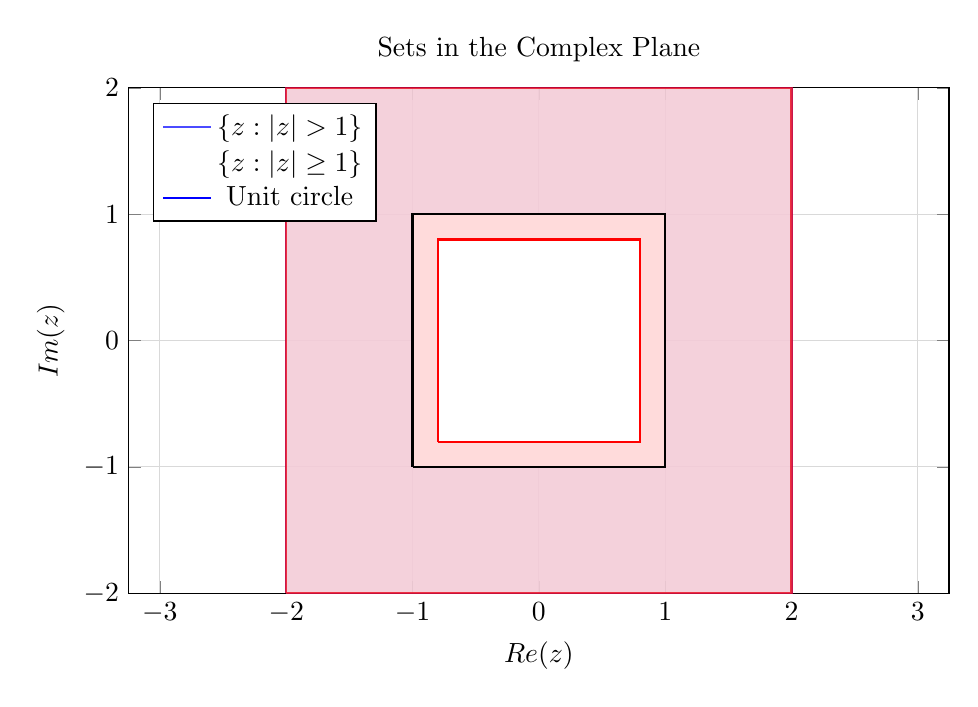
\begin{tikzpicture}
\begin{axis}[
    width=12cm,
    height=8cm,
    xlabel={$\text{Re}(z)$},
    ylabel={$\text{Im}(z)$},
    title={Sets in the Complex Plane},
    xmin=-2, xmax=2,
    ymin=-2, ymax=2,
    grid=major,
    grid style={gray!30},
    legend pos=north west,
    axis equal
]

% |z| > 1 (exterior of unit circle)
\addplot[blue, thick, fill=blue!20, opacity=0.7] coordinates {
    (-2,-2) (2,-2) (2,2) (-2,2) (-2,-2)
};
\addplot[white, thick, fill=white] coordinates {
    (-1,-1) (1,-1) (1,1) (-1,1) (-1,-1)
};
\addplot[blue, thick] coordinates {
    (-1,-1) (1,-1) (1,1) (-1,1) (-1,-1)
};
\addlegendentry{$\{z : |z| > 1\}$}

% |z| ≥ 1 (complement of open unit disk)
\addplot[red, thick, fill=red!20, opacity=0.7] coordinates {
    (-2,-2) (2,-2) (2,2) (-2,2) (-2,-2)
};
\addplot[white, thick, fill=white] coordinates {
    (-0.8,-0.8) (0.8,-0.8) (0.8,0.8) (-0.8,0.8) (-0.8,-0.8)
};
\addplot[red, thick] coordinates {
    (-0.8,-0.8) (0.8,-0.8) (0.8,0.8) (-0.8,0.8) (-0.8,-0.8)
};
\addlegendentry{$\{z : |z| \geq 1\}$}

% Unit circle
\addplot[black, thick] coordinates {
    (-1,-1) (1,-1) (1,1) (-1,1) (-1,-1)
};
\addlegendentry{Unit circle}

\end{axis}
\end{tikzpicture}
\caption{Left: $\{z : |z| > 1\}$ is open but not closed. Right: $\{z : |z| \geq 1\}$ is closed but not open.}
\end{figure}

\bigskip\noindent\textbf{Solution:}
(a) The set $\{z \in \mathbb{C} : |z| > 1\}$ has accumulation points $\{z \in \mathbb{C} : |z| \geq 1\}$. The set is open but not closed.

(b) The set $\{z \in \mathbb{C} : |z| \geq 1\}$ has accumulation points $\{z \in \mathbb{C} : |z| \geq 1\}$. The set is closed but not open.

(c) The set $\{(1/n, 1/m) : m,n \in \mathbb{N}\}$ has accumulation points $\{(1/n, 0) : n \in \mathbb{N}\} \cup \{(0, 1/m) : m \in \mathbb{N}\} \cup \{(0, 0)\}$. For $(1/k, 0)$, take $(1/k, 1/m_n)$ with $m_n \to \infty$; for $(0, 1/l)$, take $(1/n_m, 1/l)$ with $n_m \to \infty$; for $(0, 0)$, take $(1/n, 1/n)$. The set is neither open nor closed (no point is interior; closure includes accumulation points).

(d) The set $\{(x,y) : x^2 - y^2 < 1\}$ has accumulation points $\{(x,y) : x^2 - y^2 \leq 1\}$. The set is open but not closed.

(e) The set $\{(x,y) : x > 0\}$ has accumulation points $\{(x,y) : x \geq 0\}$. The set is open but not closed.

(f) The set $\{(x,y) : x \geq 0\}$ has accumulation points $\{(x,y) : x \geq 0\}$. The set is closed but not open.\qed


\begin{problembox}[3.4: Rational and Irrational Elements in Open Sets]
\begin{problemstatement}
Prove that every nonempty open set $S$ in $\mathbb{R}^1$ contains both rational and irrational numbers.
\end{problemstatement}
\end{problembox}

\noindent\textbf{Strategy:} Use the density of rational and irrational numbers in $\mathbb{R}$. Since $S$ is open, any point in $S$ has a neighborhood contained in $S$. By density, both rational and irrational numbers exist in any open interval.

\bigskip\noindent\textbf{Solution:} Let $S$ be a nonempty open set in $\mathbb{R}^1$. Since $S$ is open, for any point $x \in S$, there exists $\varepsilon > 0$ such that the open interval $(x-\varepsilon, x+\varepsilon) \subset S$.

Since the rational numbers are dense in $\mathbb{R}$, there exists a rational number $q$ in $(x-\varepsilon, x+\varepsilon)$, and thus $q \in S$.

Similarly, since the irrational numbers are also dense in $\mathbb{R}$, there exists an irrational number $r$ in $(x-\varepsilon, x+\varepsilon)$, and thus $r \in S$.

Therefore, every nonempty open set contains both rational and irrational numbers.\qed


\begin{problembox}[3.5: Open and Closed Sets in $\mathbb{R}^1$ and $\mathbb{R}^2$]
\begin{problemstatement}
Prove that the only sets in $\mathbb{R}^1$ which are both open and closed are the empty set and $\mathbb{R}^1$ itself. Is a similar statement true for $\mathbb{R}^2$?
\end{problemstatement}
\end{problembox}

\noindent\textbf{Strategy:} Use proof by contradiction. Assume there exists a non-empty proper subset that is both open and closed. Use the connectedness of $\mathbb{R}^1$ and $\mathbb{R}^2$ - if a space is connected, it cannot be split into two non-empty disjoint open sets. The key is to show that such a split would violate connectedness.

% Visualization for Exercise 3.5: Connectedness Proof
\begin{figure}[h]
\centering
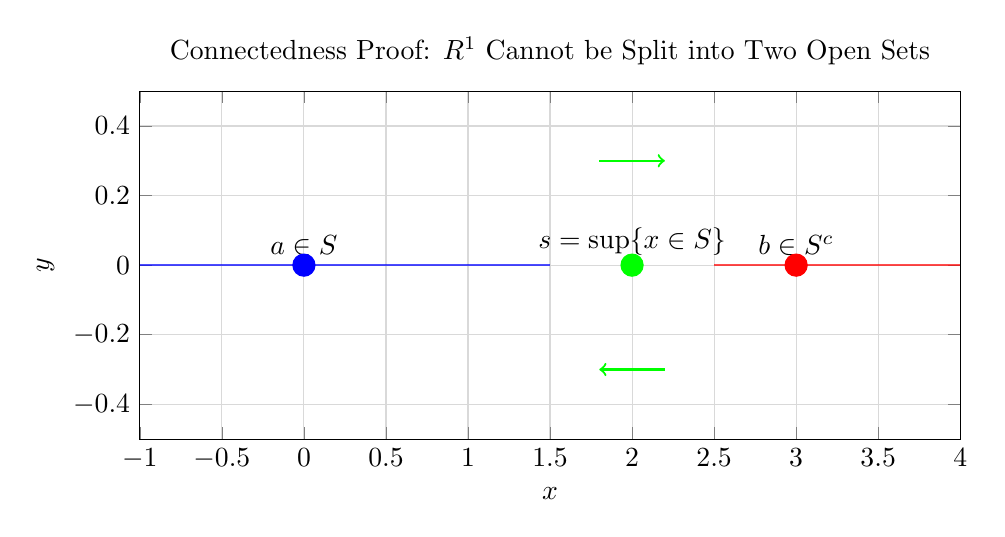
\begin{tikzpicture}
\begin{axis}[
    width=12cm,
    height=6cm,
    xlabel={$x$},
    ylabel={$y$},
    title={Connectedness Proof: $\mathbb{R}^1$ Cannot be Split into Two Open Sets},
    xmin=-1, xmax=4,
    ymin=-0.5, ymax=0.5,
    grid=major,
    grid style={gray!30},
    legend pos=north east
]

% Two hypothetical open sets
\addplot[blue, thick, fill=blue!20, opacity=0.7] coordinates {(-1,0) (1.5,0)};
\addplot[red, thick, fill=red!20, opacity=0.7] coordinates {(2.5,0) (4,0)};

% Points from each set
\addplot[blue, mark=*, mark size=4pt] coordinates {(0,0)};
\addplot[red, mark=*, mark size=4pt] coordinates {(3,0)};

% Labels
\node[above] at (axis cs:0,0) {$a \in S$};
\node[above] at (axis cs:3,0) {$b \in S^c$};

% Supremum point
\addplot[green, mark=*, mark size=4pt] coordinates {(2,0)};
\node[above] at (axis cs:2,0) {$s = \sup\{x \in S\}$};

% Contradiction arrows
\draw[->, thick, green] (axis cs:1.8,0.3) -- (axis cs:2.2,0.3);
\draw[->, thick, green] (axis cs:2.2,-0.3) -- (axis cs:1.8,-0.3);

\end{axis}
\end{tikzpicture}
\caption{Proof by contradiction that $\mathbb{R}^1$ is connected. If it could be split into two open sets, the supremum $s$ would lead to a contradiction.}
\end{figure}

\bigskip\noindent\textbf{Solution:}

\subsubsection*{Proof for $\mathbb{R}^1$}

We need to show that if a set $S$ in $\mathbb{R}^1$ is both open and closed, then $S$ must be either the empty set $\emptyset$ or all of $\mathbb{R}^1$.

Let's start by understanding what it means for a set to be both open and closed. If $S$ is open, then every point in $S$ has a small neighborhood around it that stays within $S$. If $S$ is closed, then its complement $S^c = \mathbb{R}^1 \setminus S$ is open.

Now, let's prove this by contradiction. Suppose there exists a set $S$ that is both open and closed, but $S$ is not empty and $S$ is not all of $\mathbb{R}^1$. This means:
\begin{enumerate}
\item $S$ is not empty (there's at least one point in $S$)
\item $S$ is not all of $\mathbb{R}^1$ (there's at least one point not in $S$)
\end{enumerate}

Since $S$ is not all of $\mathbb{R}^1$, its complement $S^c$ is not empty. And since $S$ is closed, $S^c$ must be open.

So we have two non-empty open sets $S$ and $S^c$ that together make up all of $\mathbb{R}^1$, and they don't overlap (they're disjoint).

Now, let's pick a point $a$ from $S$ and a point $b$ from $S^c$. Without loss of generality, assume $a < b$.

Consider the interval $[a, b]$. Since $S$ is open and contains $a$, there must be some small distance $\varepsilon_1 > 0$ such that the interval $(a - \varepsilon_1, a + \varepsilon_1)$ is completely contained in $S$.

Similarly, since $S^c$ is open and contains $b$, there must be some small distance $\varepsilon_2 > 0$ such that the interval $(b - \varepsilon_2, b + \varepsilon_2)$ is completely contained in $S^c$.

Now, let's look at the set of all points in $[a, b]$ that belong to $S$. This set has a supremum (least upper bound) because it's bounded above by $b$. Let's call this supremum $s$.

The key insight is that $s$ must belong to $S$. Here's why: if $s$ were in $S^c$, then since $S^c$ is open, there would be a small interval around $s$ that's completely in $S^c$. But this would mean there are points in $S^c$ that are larger than $s$, which contradicts the fact that $s$ is the supremum of points in $S$.

So $s$ is in $S$. But since $S$ is open, there must be a small interval around $s$ that's completely contained in $S$. This means there are points in $S$ that are larger than $s$, which again contradicts the fact that $s$ is the supremum.

This contradiction shows that our original assumption was wrong. Therefore, the only sets in $\mathbb{R}^1$ that are both open and closed are the empty set and $\mathbb{R}^1$ itself.

\subsubsection*{For $\mathbb{R}^2$}

Yes, the same statement is true for $\mathbb{R}^2$. The only subsets of $\mathbb{R}^2$ that are both open and closed are the empty set and $\mathbb{R}^2$ itself.

The proof is similar in spirit but more complex because we're working in two dimensions. The key idea is that $\mathbb{R}^2$ is "connected" - you can draw a continuous path between any two points without leaving $\mathbb{R}^2$.

If there were a non-empty proper subset $S$ of $\mathbb{R}^2$ that was both open and closed, then its complement $S^c$ would also be non-empty, open, and closed. You could then pick a point from $S$ and a point from $S^c$ and try to draw a continuous path between them. But this path would have to "jump" from one set to the other at some point, which would violate the continuity of the path.

This property is called "connectedness" - a space is connected if it cannot be split into two non-empty, disjoint, open sets. Both $\mathbb{R}^1$ and $\mathbb{R}^2$ are connected spaces.\qed


\begin{problembox}[3.6: Closed Sets as Intersection of Open Sets]
\begin{problemstatement}
Prove that every closed set in $\mathbb{R}^1$ is the intersection of a countable collection of open sets.
\end{problemstatement}
\end{problembox}

\noindent\textbf{Strategy:} Use the distance function $d(x,F) = \inf\{|x-y| : y \in F\}$ to construct open sets $G_n = \{x : d(x,F) < 1/n\}$. Show that the intersection of these open sets equals the closed set $F$ by using the fact that $d(x,F) = 0$ if and only if $x \in F$ (when $F$ is closed).

\bigskip\noindent\textbf{Solution:} Let $F$ be a closed set in $\mathbb{R}^1$. For each $n \in \mathbb{N}$, define $G_n = \{x \in \mathbb{R} : d(x,F) < 1/n\}$, where $d(x,F) = \inf\{|x-y| : y \in F\}$. Each $G_n$ is open since it's the union of open intervals.

We claim that $F = \bigcap_{n=1}^{\infty} G_n$. Clearly $F \subset \bigcap_{n=1}^{\infty} G_n$ since every point in $F$ has distance 0 to $F$.

For the reverse inclusion, let $x \in \bigcap_{n=1}^{\infty} G_n$. Then $d(x,F) < 1/n$ for all $n$, which means $d(x,F) = 0$. Since $F$ is closed, this implies $x \in F$.\qed


\begin{problembox}[3.7: Structure of Bounded Closed Sets in $\mathbb{R}^1$]
\begin{problemstatement}
Prove that a nonempty, bounded closed set $S$ in $\mathbb{R}^1$ is either a closed interval, or that $S$ can be obtained from a closed interval by removing a countable disjoint collection of open intervals whose endpoints belong to $S$.
\end{problemstatement}
\end{problembox}

\noindent\textbf{Strategy:} Use the fact that a bounded closed set has a minimum and maximum. If $S$ is not a closed interval, its complement in the minimal closed interval containing $S$ is open and can be written as a countable union of disjoint open intervals. Since $S$ is closed, the endpoints of these intervals must belong to $S$.

\bigskip\noindent\textbf{Solution:} Let $S$ be a nonempty, bounded closed set in $\mathbb{R}^1$. Let $a = \inf S$ and $b = \sup S$. Since $S$ is closed, $a, b \in S$.

If $S = [a,b]$, we're done. Otherwise, the complement $[a,b] \setminus S$ is open and can be written as a countable union of disjoint open intervals $(a_i, b_i)$. Since $S$ is closed, the endpoints $a_i, b_i$ must belong to $S$.

Therefore, $S = [a,b] \setminus \bigcup_{i=1}^{\infty} (a_i, b_i)$, which is the desired representation.\qed
\section{Open and Closed Sets in $\mathbb{R}^n$}

\subsection*{Definitions and Theorems for Section 3.2}

\begin{definition}[Open Ball]
Given a metric space $(M,d)$, the open ball centered at a point $a \in M$ with radius $r > 0$ is the set $B(a;r) = \{x \in M : d(x,a) < r\}$.
\end{definition}

\begin{definition}[Interior of a Set]
Given a set $S$ in a metric space $(M,d)$, the interior of $S$, denoted by $\text{int } S$, is the set of all interior points of $S$.
\end{definition}

\begin{theorem}[Properties of the Interior]
Let $S$ and $T$ be subsets of a metric space $(M,d)$. Then the following properties hold:
\begin{enumerate}
\item The interior $\text{int } S$ is an open set.
\item The interior $\text{int } S$ is the largest open subset of $S$.
\item The interior of the interior equals the interior: $\text{int }(\text{int } S) = \text{int } S$.
\item The interior of an intersection equals the intersection of interiors: $\text{int }(S \cap T) = \text{int } S \cap \text{int } T$.
\item The union of interiors is contained in the interior of the union: $\text{int } S \cup \text{int } T \subseteq \text{int }(S \cup T)$.
\end{enumerate}
\end{theorem}

\begin{theorem}[Interior as Union of Open Subsets]
If $S$ is a subset of $\mathbb{R}^n$, then the interior of $S$ is equal to the union of all open subsets of $\mathbb{R}^n$ that are contained in $S$.
\end{theorem}



\begin{problembox}[3.8: Open Balls and Intervals in Rn]
\begin{problemstatement}
Prove that open n-balls and n-dimensional open intervals are open sets in $\mathbb{R}^n$.
\end{problemstatement}
\end{problembox}

\noindent\textbf{Strategy:} For open balls, use the triangle inequality to show that any point in the ball has a neighborhood contained in the ball. For open intervals, use the fact that they are products of open intervals in each coordinate and show that any point has a neighborhood contained in the product.

\bigskip\noindent\textbf{Solution:} Let $B(a;r) = \{x \in \mathbb{R}^n : \|x-a\| < r\}$ be an open ball centered at $a$ with radius $r$. For any $x \in B(a;r)$, let $\varepsilon = r - \|x-a\| > 0$. Then $B(x;\varepsilon) \subset B(a;r)$ by the triangle inequality, showing $B(a;r)$ is open.

For an open interval $I = (a_1,b_1) \times \cdots \times (a_n,b_n)$, let $x = (x_1,\ldots,x_n) \in I$. For each $i$, let $\varepsilon_i = \min\{x_i - a_i, b_i - x_i\}$. Then the ball $B(x;\min\{\varepsilon_1,\ldots,\varepsilon_n\}) \subset I$, showing $I$ is open.\qed


\begin{problembox}[3.9: Interior of a Set is Open]
\begin{problemstatement}
Prove that the interior of a set in $\mathbb{R}^n$ is open in $\mathbb{R}^n$.
\end{problemstatement}
\end{problembox}

\noindent\textbf{Strategy:} Use the definition of interior point: a point is interior if it has a neighborhood contained in the set. Show that if a point is interior, then every point in a small enough neighborhood around it is also interior, making the interior set itself open.

\bigskip\noindent\textbf{Solution:} Let $S \subset \mathbb{R}^n$ and let $x \in \text{int } S$. By definition, there exists $\varepsilon > 0$ such that $B(x;\varepsilon) \subset S$.

For any $y \in B(x;\varepsilon)$, let $\delta = \varepsilon - \|y-x\| > 0$. Then $B(y;\delta) \subset B(x;\varepsilon) \subset S$, which shows that $y \in \text{int } S$.

Therefore, $B(x;\varepsilon) \subset \text{int } S$, proving that $\text{int } S$ is open.\qed


\begin{problembox}[3.10: Interior as Union of Open Subsets]
\begin{problemstatement}
If $S \subseteq \mathbb{R}^n$, prove that int $S$ is the union of all open subsets of $\mathbb{R}^n$ which are contained in $S$. This is described by saying that int $S$ is the largest open subset of $S$.
\end{problemstatement}
\end{problembox}

\noindent\textbf{Strategy:} Show two inclusions: (1) any open subset contained in $S$ is contained in int $S$ (since all its points are interior), and (2) int $S$ is contained in the union of all open subsets of $S$ (since int $S$ itself is an open subset of $S$).

\bigskip\noindent\textbf{Solution:} Let $\mathcal{U}$ be the collection of all open subsets of $\mathbb{R}^n$ contained in $S$. We need to show that $\text{int } S = \bigcup_{U \in \mathcal{U}} U$.

First, if $x \in \text{int } S$, then there exists $\varepsilon > 0$ such that $B(x;\varepsilon) \subset S$. Since $B(x;\varepsilon)$ is open and contained in $S$, we have $x \in B(x;\varepsilon) \in \mathcal{U}$, so $x \in \bigcup_{U \in \mathcal{U}} U$.

Conversely, if $x \in \bigcup_{U \in \mathcal{U}} U$, then $x \in U$ for some open set $U \subset S$. Since $U$ is open, there exists $\varepsilon > 0$ such that $B(x;\varepsilon) \subset U \subset S$, which shows $x \in \text{int } S$.

Therefore, $\text{int } S = \bigcup_{U \in \mathcal{U}} U$, proving that the interior is the largest open subset of $S$.\qed


\begin{problembox}[3.11: Interior of Intersection and Union]
\begin{problemstatement}
If $S$ and $T$ are subsets of $\mathbb{R}^n$, prove that
int$(S)$ $\cap$ int$(T)$ = int$(S \cap T)$,
and int$(S)$ $\cup$ int$(T)$ $\subseteq$ int$(S \cup T)$.
\end{problemstatement}
\end{problembox}    

\noindent\textbf{Strategy:} For the first equality, show both inclusions using the fact that if a point is interior to both sets, it has a neighborhood in their intersection. For the second inclusion, use the fact that if a point is interior to either set, it has a neighborhood in their union.

\bigskip\noindent\textbf{Solution:} For the first equality, let $x \in \text{int}(S) \cap \text{int}(T)$. Then there exist $\varepsilon_1, \varepsilon_2 > 0$ such that $B(x;\varepsilon_1) \subset S$ and $B(x;\varepsilon_2) \subset T$. Let $\varepsilon = \min\{\varepsilon_1, \varepsilon_2\}$. Then $B(x;\varepsilon) \subset S \cap T$, so $x \in \text{int}(S \cap T)$.

Conversely, if $x \in \text{int}(S \cap T)$, there exists $\varepsilon > 0$ such that $B(x;\varepsilon) \subset S \cap T$. This implies $B(x;\varepsilon) \subset S$ and $B(x;\varepsilon) \subset T$, so $x \in \text{int}(S) \cap \text{int}(T)$.

For the second inclusion, if $x \in \text{int}(S) \cup \text{int}(T)$, then $x \in \text{int}(S)$ or $x \in \text{int}(T)$. In either case, there exists $\varepsilon > 0$ such that $B(x;\varepsilon) \subset S$ or $B(x;\varepsilon) \subset T$, which implies $B(x;\varepsilon) \subset S \cup T$. Therefore, $x \in \text{int}(S \cup T)$.\qed


\begin{problembox}[3.12: Properties of Derived Set and Closure]
\begin{problemstatement}
Let $S'$ denote the derived set and $\overline{S}$ the closure of a set $S$ in $\mathbb{R}^n$. Prove that:
\begin{enumerate}[label=\alph*)]
\item $S'$ is closed in $\mathbb{R}^n$; that is, $\overline{S'} \subseteq S'$.
\item If $S \subseteq T$, then $S' \subseteq T'$.
\item $S' \cup T' = (S \cup T)'$.
\item $\overline{S} = S \cup S'$.
\item $\overline{S}$ is closed in $\mathbb{R}^n$.
\item $\overline{S}$ is the intersection of all closed subsets of $\mathbb{R}^n$ containing $S$. That is, $\overline{S}$ is the smallest closed set containing $S$.
\end{enumerate}
\end{problemstatement}
\end{problembox}

\noindent\textbf{Strategy:} Use the definitions of derived set (accumulation points) and closure (adherent points). For (a), show that accumulation points of accumulation points are accumulation points. For (b), use the subset relationship. For (c), show both inclusions using the definition. For (d), use the fact that adherent points are either in the set or accumulation points. For (e), use (a) and (d). For (f), show that closure is both contained in and contains the intersection.

\bigskip\noindent\textbf{Solution:}\\
(a) To prove $S'$ is closed, we must show that its derived set $(S')'$ is a subset of $S'$. Let $\mathbf{x} \in (S')'$. This means every neighborhood of $\mathbf{x}$ contains a point of $S'$ other than $\mathbf{x}$. Let $B(\mathbf{x}, \varepsilon)$ be an arbitrary open ball centered at $\mathbf{x}$. By definition of $(S')'$, there is a point $\mathbf{y} \in B(\mathbf{x}, \varepsilon) \cap S'$. Since $B(\mathbf{x}, \varepsilon)$ is an open set, it is a neighborhood for $\mathbf{y}$. Because $\mathbf{y} \in S'$, $\mathbf{y}$ is an accumulation point of $S$, so this neighborhood must contain infinitely many points from $S$. Thus, the ball $B(\mathbf{x}, \varepsilon)$ contains infinitely many points from $S$. As $B(\mathbf{x}, \varepsilon)$ was an arbitrary neighborhood of $\mathbf{x}$, this shows that $\mathbf{x}$ is an accumulation point of $S$, so $\mathbf{x} \in S'$. Therefore, $(S')' \subseteq S'$, which proves that $S'$ is a closed set.

(b) Let $\mathbf{x} \in S'$. Then every neighborhood of $\mathbf{x}$ contains a point $\mathbf{y} \in S$ with $\mathbf{y} \neq \mathbf{x}$. Since $S \subseteq T$, this point $\mathbf{y}$ is also in $T$. Thus, every neighborhood of $\mathbf{x}$ contains a point $\mathbf{y} \in T$ with $\mathbf{y} \neq \mathbf{x}$. This means $\mathbf{x} \in T'$. So $S' \subseteq T'$.

(c) Using (b), since $S \subseteq S \cup T$ and $T \subseteq S \cup T$, we have $S' \subseteq (S \cup T)'$ and $T' \subseteq (S \cup T)'$. Therefore, $S' \cup T' \subseteq (S \cup T)'$. For the reverse inclusion, let $\mathbf{x} \in (S \cup T)'$. If $\mathbf{x} \notin S'$, then there is a neighborhood of $\mathbf{x}$ that contains no points of $S$ (other than possibly $\mathbf{x}$). But since $\mathbf{x} \in (S \cup T)'$, this neighborhood must contain infinitely many points from $S \cup T$. These points must therefore come from $T$. This implies $\mathbf{x} \in T'$. So, every point in $(S \cup T)'$ must be in $S'$ or $T'$. Thus, $(S \cup T)' \subseteq S' \cup T'$.

(d) The closure $\overline{S}$ consists of all points adherent to $S$. A point $\mathbf{x}$ is adherent to $S$ if every neighborhood of $\mathbf{x}$ intersects $S$.
($\overline{S} \subseteq S \cup S'$): Let $\mathbf{x} \in \overline{S}$. If $\mathbf{x} \in S$, we are done. If $\mathbf{x} \notin S$, then every neighborhood of $\mathbf{x}$ must contain a point from $S$, and that point cannot be $\mathbf{x}$. This is the definition of an accumulation point, so $\mathbf{x} \in S'$. Thus $\overline{S} \subseteq S \cup S'$.
($S \cup S' \subseteq \overline{S}$): If $\mathbf{x} \in S$, it is in $\overline{S}$ because every neighborhood contains $\mathbf{x}$. If $\mathbf{x} \in S'$, every neighborhood contains a point of $S$, so $\mathbf{x}$ is an adherent point. Thus $S' \subseteq \overline{S}$. This gives $S \cup S' \subseteq \overline{S}$.

(e) To prove $\overline{S}$ is closed, we show its derived set $(\overline{S})'$ is a subset of $\overline{S}$. From (d), $\overline{S} = S \cup S'$. Using (c), we get $(\overline{S})' = (S \cup S')' = S' \cup (S')'$. From (a), $S'$ is closed, which means $(S')' \subseteq S'$. Therefore, $(\overline{S})' \subseteq S' \cup S' = S'$. Since $S' \subseteq S \cup S' = \overline{S}$, we have $(\overline{S})' \subseteq \overline{S}$. This proves that $\overline{S}$ is closed.

(f) Let $\mathcal{C}$ be the collection of all closed sets containing $S$. Let $C_{min} = \bigcap_{F \in \mathcal{C}} F$.
($\overline{S} \subseteq C_{min}$): Let $F$ be any set in $\mathcal{C}$. Then $F$ is closed and $S \subseteq F$. The closure of a set is the smallest closed set containing it, so we must have $\overline{S} \subseteq F$. Since this holds for all $F \in \mathcal{C}$, we have $\overline{S} \subseteq \bigcap_{F \in \mathcal{C}} F = C_{min}$.
($C_{min} \subseteq \overline{S}$): By part (e), $\overline{S}$ is a closed set. It also contains $S$. Therefore, $\overline{S}$ is one of the sets in the collection $\mathcal{C}$. The intersection of all sets in $\mathcal{C}$ must be a subset of any particular member, so $C_{min} \subseteq \overline{S}$.
Thus, $\overline{S} = C_{min}$.\qed


\begin{problembox}[3.13: Closure under Intersection of Sets]
\begin{problemstatement}
Let $S$ and $T$ be subsets of $\mathbb{R}^k$. Prove that $\overline{S \cup T} = \overline{S} \cup \overline{T}$ and that $\overline{S \cap T} \subseteq \overline{S} \cap \overline{T}$ if $S$ is open.

\textit{NOTE.} The statements in Exercises 3.9 through 3.13 are true in any metric space.
\end{problemstatement}
\end{problembox}

\noindent\textbf{Strategy:} For the union, use the monotonicity of closure and show both inclusions. For the intersection, use the fact that if a point is adherent to the intersection, it's adherent to both sets. The openness of $S$ is not needed for the intersection inclusion.

\noindent\textbf{Proof.}
We use only the definition of closure via adherent points.

For the union, first note $S\subseteq S\cup T$ and $T\subseteq S\cup T$, so by monotonicity of closure,
\[\overline S\subseteq \overline{S\cup T},\qquad \overline T\subseteq \overline{S\cup T},\]
whence $\overline S\cup\overline T\subseteq \overline{S\cup T}$. Conversely, if $x\in \overline{S\cup T}$, then every neighborhood of $x$ meets $S\cup T$, hence meets $S$ or $T$. Therefore $x\in\overline S\cup\overline T$. Thus $\overline{S\cup T}=\overline S\cup\overline T$.

For the intersection, if $x\in \overline{S\cap T}$ then every neighborhood of $x$ meets $S\cap T$, hence meets both $S$ and $T$. Therefore $x\in\overline S$ and $x\in\overline T$, so
\[\overline{S\cap T}\subseteq \overline S\cap \overline T.\]
This inclusion holds without any hypothesis on $S$.



\begin{problembox}[3.14: Properties of Convex Sets]
\begin{problemstatement}
A set \( S \) in \( \mathbb{R}^n \) is called convex if, for every pair of points \( x \) and \( y \) in \( S \) and every real \( \theta \) satisfying \( 0 < \theta < 1 \), we have \( \theta x + (1 - \theta)y \in S \). Interpret this statement geometrically (in \( \mathbb{R}^2 \) and \( \mathbb{R}^3 \)) and prove that:
\begin{enumerate}[label=\alph*)]
\item Every \( n \)-ball in \( \mathbb{R}^n \) is convex.
\item Every \( n \)-dimensional open interval is convex.
\item The interior of a convex set is convex.
\item The closure of a convex set is convex.
\end{enumerate}
\end{problemstatement}
\end{problembox}

\noindent\textbf{Strategy:} Use the triangle inequality for (a), coordinate-wise inequalities for (b), and the fact that convex combinations preserve neighborhoods for (c) and (d). For (c), show that if two points are interior, their convex combination has a neighborhood in the set. For (d), use sequences and the fact that convex combinations are continuous.

% Visualization for Exercise 3.14: Convex Sets
\begin{figure}[h]
\centering
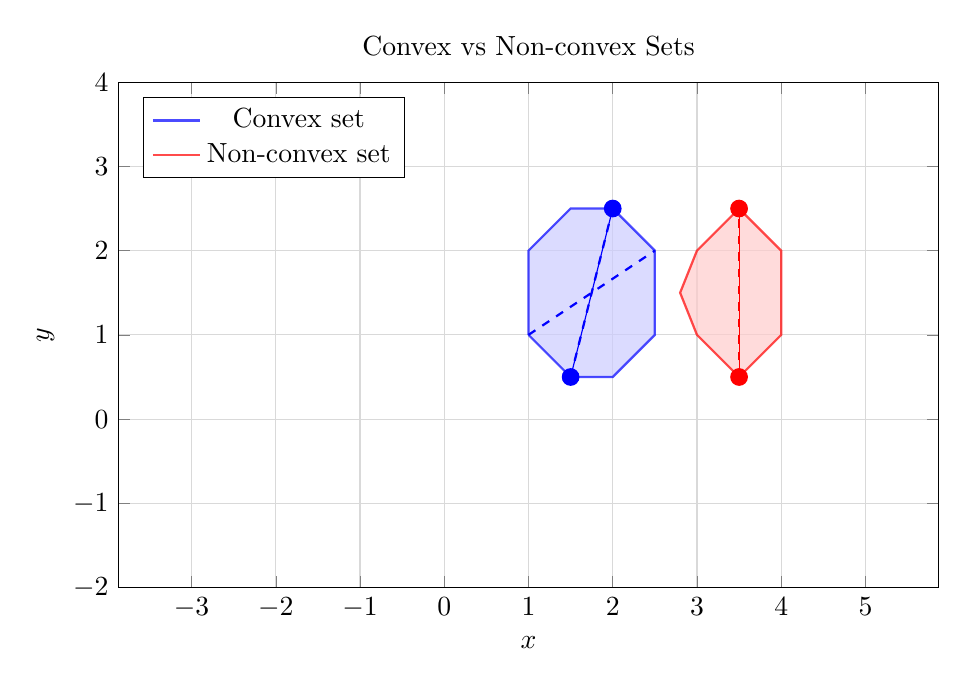
\begin{tikzpicture}
\begin{axis}[
    width=12cm,
    height=8cm,
    xlabel={$x$},
    ylabel={$y$},
    title={Convex vs Non-convex Sets},
    xmin=-2, xmax=4,
    ymin=-2, ymax=4,
    grid=major,
    grid style={gray!30},
    legend pos=north west,
    axis equal
]

% Convex set (circle)
\addplot[blue, thick, fill=blue!20, opacity=0.7] coordinates {
    (1,1) (1.5,0.5) (2,0.5) (2.5,1) (2.5,2) (2,2.5) (1.5,2.5) (1,2) (1,1)
};
\addlegendentry{Convex set}

% Non-convex set (crescent)
\addplot[red, thick, fill=red!20, opacity=0.7] coordinates {
    (3,1) (3.5,0.5) (4,1) (4,2) (3.5,2.5) (3,2) (2.8,1.5) (3,1)
};
\addlegendentry{Non-convex set}

% Line segments showing convexity
\addplot[blue, dashed, thick] coordinates {(1.5,0.5) (2,2.5)};
\addplot[blue, dashed, thick] coordinates {(1,1) (2.5,2)};

% Line segment showing non-convexity
\addplot[red, dashed, thick] coordinates {(3.5,0.5) (3.5,2.5)};

% Points
\addplot[blue, mark=*, mark size=3pt] coordinates {(1.5,0.5) (2,2.5)};
\addplot[red, mark=*, mark size=3pt] coordinates {(3.5,0.5) (3.5,2.5)};

\end{axis}
\end{tikzpicture}
\caption{Left: A convex set where any line segment between two points lies entirely within the set. Right: A non-convex set where some line segments between points extend outside the set.}
\end{figure}

\bigskip\noindent\textbf{Solution:} Geometrically, a set is convex if the line segment joining any two points in the set lies entirely within the set.

(a) Let $B(a;r)$ be an $n$-ball and $x, y \in B(a;r)$. For $0 < \theta < 1$, let $z = \theta x + (1-\theta)y$. Then $\|z-a\| = \|\theta(x-a) + (1-\theta)(y-a)\| \leq \theta\|x-a\| + (1-\theta)\|y-a\| < \theta r + (1-\theta)r = r$, so $z \in B(a;r)$.

(b) Let $I = (a_1,b_1) \times \cdots \times (a_n,b_n)$ be an open interval and $x, y \in I$. For $0 < \theta < 1$, let $z = \theta x + (1-\theta)y$. For each $i$, we have $a_i < x_i, y_i < b_i$, so $a_i < \theta x_i + (1-\theta)y_i < b_i$. Therefore, $z \in I$.

(c) Let $S$ be convex and $x, y \in \text{int } S$. There exist $\varepsilon_1, \varepsilon_2 > 0$ such that $B(x;\varepsilon_1) \subset S$ and $B(y;\varepsilon_2) \subset S$. Let $\varepsilon = \min\{\varepsilon_1, \varepsilon_2\}$. For $0 < \theta < 1$, let $z = \theta x + (1-\theta)y$. If $w \in B(z;\varepsilon)$, then $\|w-z\| < \varepsilon$. Let $u = w - z + x$ and $v = w - z + y$. Then $\|u-x\| = \|v-y\| = \|w-z\| < \varepsilon$, so $u, v \in S$. Since $S$ is convex, $w = \theta u + (1-\theta)v \in S$. Therefore, $B(z;\varepsilon) \subset S$, so $z \in \text{int } S$.

(d) Let $S$ be convex and $x, y \in \overline{S}$. There exist sequences $\{x_n\}, \{y_n\} \subset S$ converging to $x, y$ respectively. For $0 < \theta < 1$, let $z = \theta x + (1-\theta)y$ and $z_n = \theta x_n + (1-\theta)y_n$. Since $S$ is convex, $z_n \in S$ for all $n$. Since $z_n \to z$, we have $z \in \overline{S}$.\qed


\begin{problembox}[3.15: Accumulation Points of Intersections and Unions]
\begin{problemstatement}
Let $\mathcal{F}$ be a collection of sets in $\mathbb{R}^k$, and let $S = \bigcup_{A \in \mathcal{F}} A$ and $T = \bigcap_{A \in \mathcal{F}} A$. For each of the following statements, either give a proof or exhibit a counterexample:
\begin{enumerate}[label=\alph*)]
\item If $\mathbf{x}$ is an accumulation point of $T$, then $\mathbf{x}$ is an accumulation point of each set $A$ in $\mathcal{F}$.
\item If $\mathbf{x}$ is an accumulation point of $S$, then $\mathbf{x}$ is an accumulation point of at least one set $A$ in $\mathcal{F}$.
\end{enumerate}
\end{problemstatement}
\end{problembox}

\noindent\textbf{Strategy:} For (a), use the fact that if a point is in the intersection, it's in every set, so accumulation points of the intersection must be accumulation points of each set. For (b), consider whether the collection is finite or infinite - for infinite collections, construct a counterexample using singletons.

\bigskip\noindent\textbf{Solution:}\\
(a) This statement is \textbf{true}.\\
\bigskip\noindent\textbf{Solution:} Let $\mathbf{x}$ be an accumulation point of $T$. This means that for any $\varepsilon > 0$, the ball $B(\mathbf{x}; \varepsilon)$ contains a point $\mathbf{y} \in T$ such that $\mathbf{y} \neq \mathbf{x}$. By definition, $T = \bigcap_{A \in \mathcal{F}} A$. So, if $\mathbf{y} \in T$, then $\mathbf{y} \in A$ for every set $A$ in the collection $\mathcal{F}$. Therefore, for any $\varepsilon > 0$, the ball $B(\mathbf{x}; \varepsilon)$ contains a point $\mathbf{y} \in A$ (for every $A \in \mathcal{F}$) with $\mathbf{y} \neq \mathbf{x}$. This is precisely the definition of $\mathbf{x}$ being an accumulation point of $A$. Thus, $\mathbf{x}$ is an accumulation point of each set $A \in \mathcal{F}$.

(b) This statement is \textbf{false} for an infinite collection $\mathcal{F}$.\\
\textbf{Counterexample:} Let the collection of sets in $\mathbb{R}^1$ be $\mathcal{F} = \{A_n : n \in \mathbb{N}\}$ where each set $A_n$ is a singleton: $A_n = \{1/n\}$.
The union is the set $S = \bigcup_{n=1}^{\infty} A_n = \{1, 1/2, 1/3, \dots\}$.
The set $S$ has exactly one accumulation point: $0$, since the sequence of points converges to $0$.
However, none of the individual sets $A_n$ have any accumulation points, as they each contain only a single isolated point.
Thus, $0$ is an accumulation point of $S$, but not of any set $A_n$ in the collection $\mathcal{F}$.

\textit{(Note: The statement is true if the collection $\mathcal{F}$ is finite. If $\mathbf{x}$ is an accumulation point of a finite union $S = A_1 \cup \dots \cup A_m$, then any neighborhood of $\mathbf{x}$ contains infinitely many points from $S$. By the pigeonhole principle, at least one of the sets $A_i$ must contribute infinitely many of these points, making $\mathbf{x}$ an accumulation point of that $A_i$.)}\qed


\begin{problembox}[3.16: Rationals  Not a Countable Intersection of Open Sets]
\begin{problemstatement}
Prove that the set \( S \) of rational numbers in the interval \( (0, 1) \) cannot be expressed as the intersection of a countable collection of open sets. 

\textit{Hint.} Write \( S = \{x_1, x_2, \ldots\} \), assume \( S = \bigcap_{k=1}^{\infty} S_k \), where each \( S_k \) is open, and construct a sequence \( (Q_n) \) of closed intervals such that \( Q_{n+1} \subseteq Q_n \subseteq S_n \) and such that \( x_n \notin Q_n \). Then use the Cantor intersection theorem to obtain a contradiction.
\end{problemstatement}
\end{problembox}

\noindent\textbf{Strategy:} Use proof by contradiction. Assume the rationals can be written as a countable intersection of open sets. Enumerate the rationals and construct nested closed intervals that exclude each rational one by one. Use the Cantor intersection theorem to find a point in the intersection that cannot be rational, creating a contradiction.

% Visualization for Exercise 3.16: Cantor Intersection Theorem
\begin{figure}[h]
\centering
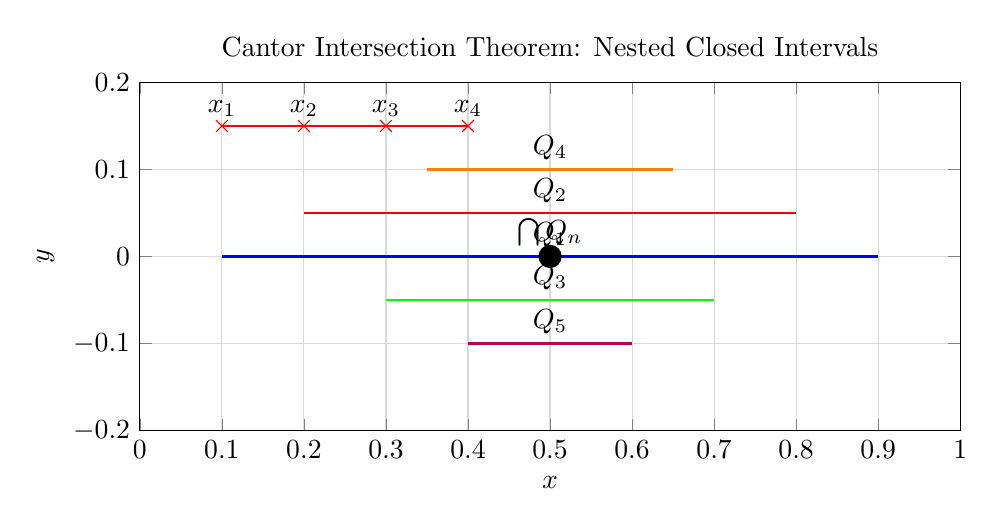
\begin{tikzpicture}
\begin{axis}[
    width=12cm,
    height=6cm,
    xlabel={$x$},
    ylabel={$y$},
    title={Cantor Intersection Theorem: Nested Closed Intervals},
    xmin=0, xmax=1,
    ymin=-0.2, ymax=0.2,
    grid=major,
    grid style={gray!30},
    legend pos=north east
]

% Nested closed intervals
\addplot[blue, thick] coordinates {(0.1,0) (0.9,0)};
\addplot[red, thick] coordinates {(0.2,0.05) (0.8,0.05)};
\addplot[green, thick] coordinates {(0.3,-0.05) (0.7,-0.05)};
\addplot[orange, thick] coordinates {(0.35,0.1) (0.65,0.1)};
\addplot[purple, thick] coordinates {(0.4,-0.1) (0.6,-0.1)};

% Labels
\node[above] at (axis cs:0.5,0) {$Q_1$};
\node[above] at (axis cs:0.5,0.05) {$Q_2$};
\node[above] at (axis cs:0.5,-0.05) {$Q_3$};
\node[above] at (axis cs:0.5,0.1) {$Q_4$};
\node[above] at (axis cs:0.5,-0.1) {$Q_5$};

% Intersection point
\addplot[black, mark=*, mark size=4pt] coordinates {(0.5,0)};
\node[above] at (axis cs:0.5,0) {$\bigcap Q_n$};

% Excluded rationals
\addplot[red, mark=x, mark size=3pt] coordinates {(0.1,0.15) (0.2,0.15) (0.3,0.15) (0.4,0.15)};
\node[above] at (axis cs:0.1,0.15) {$x_1$};
\node[above] at (axis cs:0.2,0.15) {$x_2$};
\node[above] at (axis cs:0.3,0.15) {$x_3$};
\node[above] at (axis cs:0.4,0.15) {$x_4$};

\end{axis}
\end{tikzpicture}
\caption{The Cantor intersection theorem: nested closed intervals $Q_n$ exclude rationals $x_n$ one by one, but their intersection must contain a point that cannot be any of the excluded rationals.}
\end{figure}

\bigskip\noindent\textbf{Solution:} The strategy is to use a proof by contradiction. We'll assume that the rationals can be written as a countable intersection of open sets, then construct a nested sequence of closed intervals that excludes each rational number one by one. This will lead to a point that must be in the intersection (by the Cantor intersection theorem) but cannot be any of the rational numbers we've excluded, creating a contradiction.

Suppose for contradiction that $S = \bigcap_{k=1}^{\infty} S_k$ where each $S_k$ is open. Let $S = \{x_1, x_2, \ldots\}$ be an enumeration of the rationals in $(0,1)$.

For each $n$, since $S_n$ is open and contains all rationals in $(0,1)$, we can find a closed interval $Q_n \subset S_n$ such that $x_n \notin Q_n$. Here's why this is possible: Since $S_n$ is open, for any point $y \in S_n$ that is not $x_n$, there exists an open interval around $y$ that is entirely contained in $S_n$. We can choose a point $y \in S_n$ that is close to but not equal to $x_n$, and then take a small closed interval around $y$ that stays within $S_n$ but excludes $x_n$. For example, if $x_n$ is not at the boundary of $S_n$, we can find a point $y \in S_n$ with $y < x_n$ and take $Q_n = [y - \varepsilon, y + \varepsilon]$ for some small $\varepsilon > 0$ such that $x_n > y + \varepsilon$. We can arrange that $Q_{n+1} \subseteq Q_n$ by taking $Q_{n+1} = Q_n \cap I_{n+1}$ where $I_{n+1}$ is a closed interval in $S_{n+1}$ that doesn't contain $x_{n+1}$.

By the Cantor intersection theorem, $\bigcap_{n=1}^{\infty} Q_n$ is nonempty. Let $x \in \bigcap_{n=1}^{\infty} Q_n$. Then $x \in \bigcap_{k=1}^{\infty} S_k = S$, so $x$ is rational. But $x \neq x_n$ for any $n$ since $x_n \notin Q_n$ for each $n$. This contradicts the fact that $S$ contains all rationals in $(0,1)$.\qed
\section{Covering Theorems in $\mathbb{R}^n$}

\subsection*{Definitions and Theorems for Section 3.3}

\begin{definition}[Open Cover]
An open cover of a set $S$ in a metric space $(M,d)$ is a collection of open sets whose union contains $S$.
\end{definition}

\begin{definition}[Compact Set]
A set $S$ in a metric space $(M,d)$ is said to be compact if every open cover of $S$ has a finite subcover.
\end{definition}

\begin{definition}[Isolated Point]
A point $x$ in a set $S$ is said to be an isolated point of $S$ if there exists a neighborhood of $x$ that contains no other points of $S$.
\end{definition}

\begin{definition}[Separable Space]
A metric space $(M,d)$ is said to be separable if it contains a countable dense subset.
\end{definition}

\begin{theorem}[Lindelöf Property]
Every separable metric space has the Lindelöf property: every open cover has a countable subcover.
\end{theorem}

\begin{theorem}[Countability of Isolated Points]
The collection of isolated points of any subset of $\mathbb{R}^n$ is countable.
\end{theorem}

\begin{theorem}[Countability via Local Countability]
If every point in a set $S$ has a neighborhood whose intersection with $S$ is countable, then $S$ is countable.
\end{theorem}



\begin{problembox}[3.17: Countability of Isolated Points]
\begin{problemstatement}
If \( S \subseteq \mathbb{R}^n \), prove that the collection of isolated points of \( S \) is countable.
\end{problemstatement}
\end{problembox}

\noindent\textbf{Strategy:} Use the fact that isolated points have disjoint neighborhoods. For each isolated point, take a smaller ball (half the radius) and show these balls are pairwise disjoint. Then use the separability of $\mathbb{R}^n$ (it has a countable dense subset) to inject the isolated points into this countable set.

% Visualization for Exercise 3.17: Isolated Points
\begin{figure}[h]
\centering
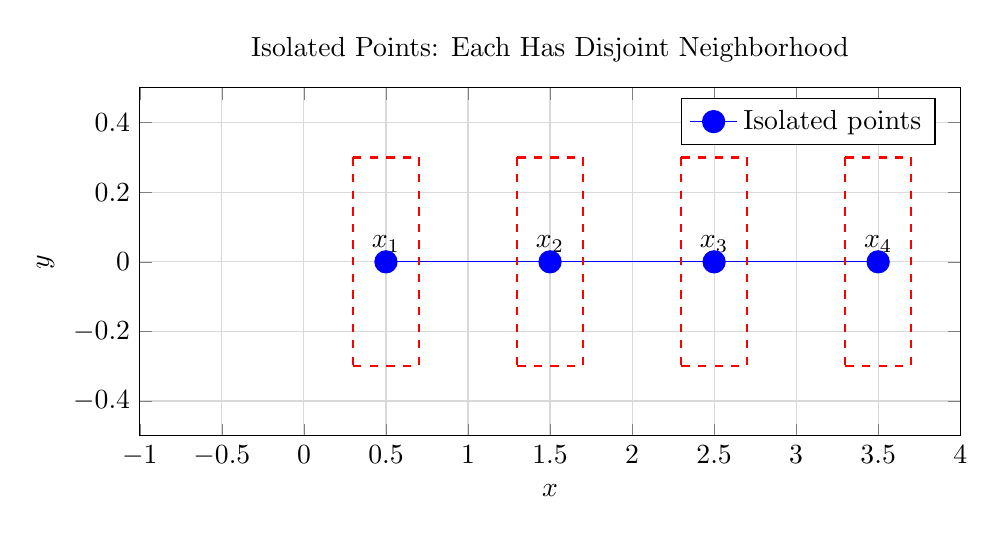
\begin{tikzpicture}
\begin{axis}[
    width=12cm,
    height=6cm,
    xlabel={$x$},
    ylabel={$y$},
    title={Isolated Points: Each Has Disjoint Neighborhood},
    xmin=-1, xmax=4,
    ymin=-0.5, ymax=0.5,
    grid=major,
    grid style={gray!30},
    legend pos=north east
]

% Isolated points
\addplot[blue, mark=*, mark size=4pt] coordinates {
    (0.5,0) (1.5,0) (2.5,0) (3.5,0)
};
\addlegendentry{Isolated points}

% Neighborhoods around each point
\addplot[red, dashed, thick] coordinates {(0.3,0.3) (0.7,0.3)};
\addplot[red, dashed, thick] coordinates {(0.3,-0.3) (0.7,-0.3)};
\addplot[red, dashed, thick] coordinates {(0.3,0.3) (0.3,-0.3)};
\addplot[red, dashed, thick] coordinates {(0.7,0.3) (0.7,-0.3)};

\addplot[red, dashed, thick] coordinates {(1.3,0.3) (1.7,0.3)};
\addplot[red, dashed, thick] coordinates {(1.3,-0.3) (1.7,-0.3)};
\addplot[red, dashed, thick] coordinates {(1.3,0.3) (1.3,-0.3)};
\addplot[red, dashed, thick] coordinates {(1.7,0.3) (1.7,-0.3)};

\addplot[red, dashed, thick] coordinates {(2.3,0.3) (2.7,0.3)};
\addplot[red, dashed, thick] coordinates {(2.3,-0.3) (2.7,-0.3)};
\addplot[red, dashed, thick] coordinates {(2.3,0.3) (2.3,-0.3)};
\addplot[red, dashed, thick] coordinates {(2.7,0.3) (2.7,-0.3)};

\addplot[red, dashed, thick] coordinates {(3.3,0.3) (3.7,0.3)};
\addplot[red, dashed, thick] coordinates {(3.3,-0.3) (3.7,-0.3)};
\addplot[red, dashed, thick] coordinates {(3.3,0.3) (3.3,-0.3)};
\addplot[red, dashed, thick] coordinates {(3.7,0.3) (3.7,-0.3)};

% Labels
\node[above] at (axis cs:0.5,0) {$x_1$};
\node[above] at (axis cs:1.5,0) {$x_2$};
\node[above] at (axis cs:2.5,0) {$x_3$};
\node[above] at (axis cs:3.5,0) {$x_4$};

\end{axis}
\end{tikzpicture}
\caption{Isolated points have disjoint neighborhoods, allowing them to be mapped injectively into a countable dense subset, proving countability.}
\end{figure}

\bigskip\noindent\textbf{Solution:}\\
Let $I$ be the set of isolated points of $S$. By definition, for each point $\mathbf{x} \in I$, there exists a radius $\varepsilon_{\mathbf{x}} > 0$ such that the open ball $B(\mathbf{x}; \varepsilon_{\mathbf{x}})$ contains no other point of $S$; that is, $B(\mathbf{x}; \varepsilon_{\mathbf{x}}) \cap S = \{\mathbf{x}\}$.

Consider the collection of smaller open balls $\mathcal{C} = \{ B(\mathbf{x}; \varepsilon_{\mathbf{x}}/2) : \mathbf{x} \in I \}$. We claim these balls are pairwise disjoint.
To prove this, let $\mathbf{x}_1$ and $\mathbf{x}_2$ be two distinct points in $I$. Suppose their corresponding balls in $\mathcal{C}$ have a point $\mathbf{y}$ in common. Then $d(\mathbf{x}_1, \mathbf{y}) < \varepsilon_{\mathbf{x}_1}/2$ and $d(\mathbf{x}_2, \mathbf{y}) < \varepsilon_{\mathbf{x}_2}/2$.
By the triangle inequality:
$$d(\mathbf{x}_1, \mathbf{x}_2) \le d(\mathbf{x}_1, \mathbf{y}) + d(\mathbf{y}, \mathbf{x}_2) < \frac{\varepsilon_{\mathbf{x}_1}}{2} + \frac{\varepsilon_{\mathbf{x}_2}}{2}$$
Assuming, without loss of generality, that $\varepsilon_{\mathbf{x}_1} \le \varepsilon_{\mathbf{x}_2}$, we get $d(\mathbf{x}_1, \mathbf{x}_2) < \varepsilon_{\mathbf{x}_2}/2 + \varepsilon_{\mathbf{x}_2}/2 = \varepsilon_{\mathbf{x}_2}$.
This implies that $\mathbf{x}_1 \in B(\mathbf{x}_2; \varepsilon_{\mathbf{x}_2})$. But $\mathbf{x}_1 \in S$ and $\mathbf{x}_1 \neq \mathbf{x}_2$. This contradicts the fact that $B(\mathbf{x}_2; \varepsilon_{\mathbf{x}_2})$ contains only one point from $S$, namely $\mathbf{x}_2$.
Therefore, the balls in the collection $\mathcal{C}$ must be pairwise disjoint.

Now we use the fact that $\mathbb{R}^n$ is \textbf{separable}, meaning it contains a countable dense subset, such as $\mathbb{Q}^n$ (the set of points with rational coordinates).
Since each ball in $\mathcal{C}$ is a non-empty open set, each must contain at least one point from the dense set $\mathbb{Q}^n$. Because the balls in $\mathcal{C}$ are disjoint, each ball must contain a \textit{different} rational point.
This allows us to define an injective (one-to-one) function from the set of isolated points $I$ to the countable set $\mathbb{Q}^n$ (by mapping each $\mathbf{x} \in I$ to a rational point in $B(\mathbf{x}; \varepsilon_{\mathbf{x}}/2)$). A set that can be mapped injectively into a countable set must itself be countable.
Thus, the set of isolated points $I$ is countable.\qed


\begin{problembox}[3.18: Countable Covering of the First Quadrant]
\begin{problemstatement}
Prove that the set of open disks in the \(xy\)-plane with center at \( (x, x) \) and radius \( x > 0 \), where \( x \) is rational, is a countable covering of the set \( \{(x, y) : x > 0, y > 0\} \).
\end{problemstatement}
\end{problembox}

\noindent\textbf{Strategy:} Show that the collection is countable (since rationals are countable) and that it covers the first quadrant. For any point $(x,y)$ in the first quadrant, find a rational $q$ such that the disk centered at $(q,q)$ with radius $q$ contains $(x,y)$. Use the distance formula and density of rationals.

% Visualization for Exercise 3.18: Countable Covering
\begin{figure}[h]
\centering
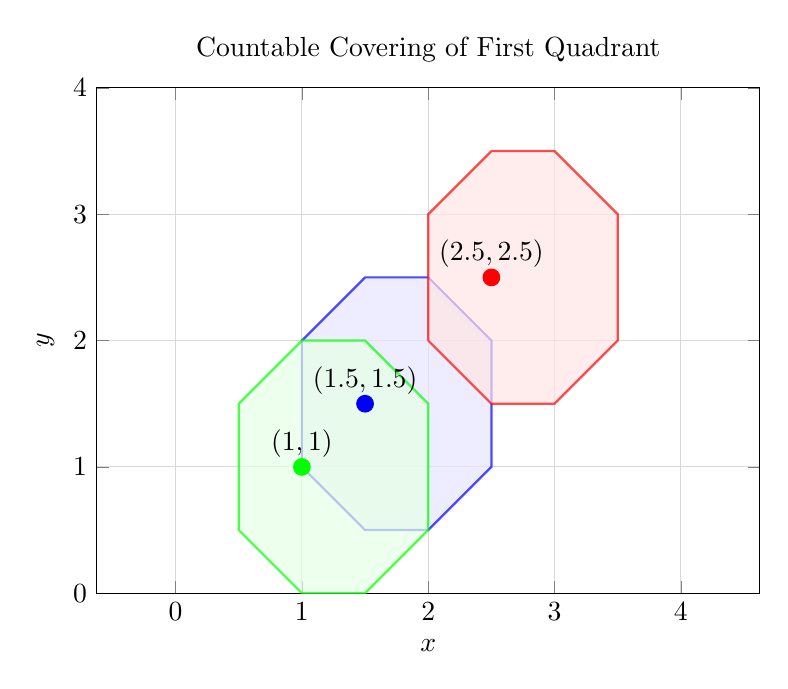
\begin{tikzpicture}
\begin{axis}[
    width=10cm,
    height=8cm,
    xlabel={$x$},
    ylabel={$y$},
    title={Countable Covering of First Quadrant},
    xmin=0, xmax=4,
    ymin=0, ymax=4,
    grid=major,
    grid style={gray!30},
    legend pos=north west,
    axis equal
]

% Several disks with rational centers
\addplot[blue, thick, fill=blue!10, opacity=0.7] coordinates {
    (1,1) (1.5,0.5) (2,0.5) (2.5,1) (2.5,2) (2,2.5) (1.5,2.5) (1,2) (1,1)
};
\addplot[red, thick, fill=red!10, opacity=0.7] coordinates {
    (2,2) (2.5,1.5) (3,1.5) (3.5,2) (3.5,3) (3,3.5) (2.5,3.5) (2,3) (2,2)
};
\addplot[green, thick, fill=green!10, opacity=0.7] coordinates {
    (0.5,0.5) (1,0) (1.5,0) (2,0.5) (2,1.5) (1.5,2) (1,2) (0.5,1.5) (0.5,0.5)
};

% Center points
\addplot[blue, mark=*, mark size=3pt] coordinates {(1.5,1.5)};
\addplot[red, mark=*, mark size=3pt] coordinates {(2.5,2.5)};
\addplot[green, mark=*, mark size=3pt] coordinates {(1,1)};

% Labels
\node[above] at (axis cs:1.5,1.5) {$(1.5, 1.5)$};
\node[above] at (axis cs:2.5,2.5) {$(2.5, 2.5)$};
\node[above] at (axis cs:1,1) {$(1, 1)$};

\end{axis}
\end{tikzpicture}
\caption{Countable covering of the first quadrant using disks centered at rational points $(q,q)$ with radius $q$.}
\end{figure}

\bigskip\noindent\textbf{Solution:}\\
Let $\mathcal{F}$ be the collection of open disks $B((q,q); q)$ where $q \in \mathbb{Q}$ and $q > 0$. Since $\mathbb{Q}$ is countable, the collection $\mathcal{F}$ is countable. We need to show that $\mathcal{F}$ covers the first quadrant $S = \{(x, y) : x > 0, y > 0\}$.

Let $(x, y)$ be an arbitrary point in $S$. We need to find a rational number $q > 0$ such that the disk $B((q,q); q)$ contains $(x, y)$. The condition for this is:
$$\sqrt{(x-q)^2 + (y-q)^2} < q$$
Since both sides are positive, we can square the inequality:
$$(x-q)^2 + (y-q)^2 < q^2$$
$$x^2 - 2xq + q^2 + y^2 - 2yq + q^2 < q^2$$
$$q^2 - 2(x+y)q + (x^2+y^2) < 0$$
Let $f(q) = q^2 - 2(x+y)q + (x^2+y^2)$. We are looking for a rational $q > 0$ that makes this quadratic expression negative. The graph of $z=f(q)$ is an upward-opening parabola. It will be negative between its roots. The roots are found using the quadratic formula:
$$q = \frac{2(x+y) \pm \sqrt{4(x+y)^2 - 4(x^2+y^2)}}{2} = (x+y) \pm \sqrt{(x+y)^2 - (x^2+y^2)}$$
$$q = (x+y) \pm \sqrt{2xy}$$
Let the roots be $q_1 = (x+y) - \sqrt{2xy}$ and $q_2 = (x+y) + \sqrt{2xy}$. Since $x,y > 0$, the term $\sqrt{2xy}$ is real and positive, so $q_1 < q_2$. The interval $(q_1, q_2)$ is non-empty.
Since the rational numbers are dense in $\mathbb{R}$, we can always find a rational number $q$ in this interval: $q_1 < q < q_2$. For any such $q$, the inequality $f(q) < 0$ holds.

We must also ensure that we can choose $q$ to be positive. The product of the roots is $q_1 q_2 = x^2+y^2 > 0$. Since $q_2 = (x+y) + \sqrt{2xy}$ is clearly positive, the other root $q_1$ must also be positive.
Since the interval $(q_1, q_2)$ consists of positive numbers and contains a rational number, we can always find a suitable rational $q > 0$.
Thus, for any point $(x,y)$ in the first quadrant, we can find a disk in $\mathcal{F}$ that contains it. The countable collection $\mathcal{F}$ therefore covers the first quadrant.\qed


\begin{problembox}[3.19: Non-Finite Subcover of \(0,1\)]
\begin{problemstatement}
The collection \( \mathcal{F} \) of open intervals of the form \( (1/n, 2/n) \), where \( n = 2, 3, \ldots \), is an open covering of the open interval \( (0, 1) \). Prove (without using Theorem 3.31) that no finite subcollection of \( \mathcal{F} \) covers \( (0, 1) \).
\end{problemstatement}
\end{problembox}

\noindent\textbf{Strategy:} Take any finite subcollection and find the maximum denominator $N$. Show that the interval $(0, 1/N)$ is not covered by any interval in the finite subcollection, since the leftmost interval is $(1/N, 2/N)$.

% Visualization for Exercise 3.19: Non-Finite Subcover
\begin{figure}[h]
\centering
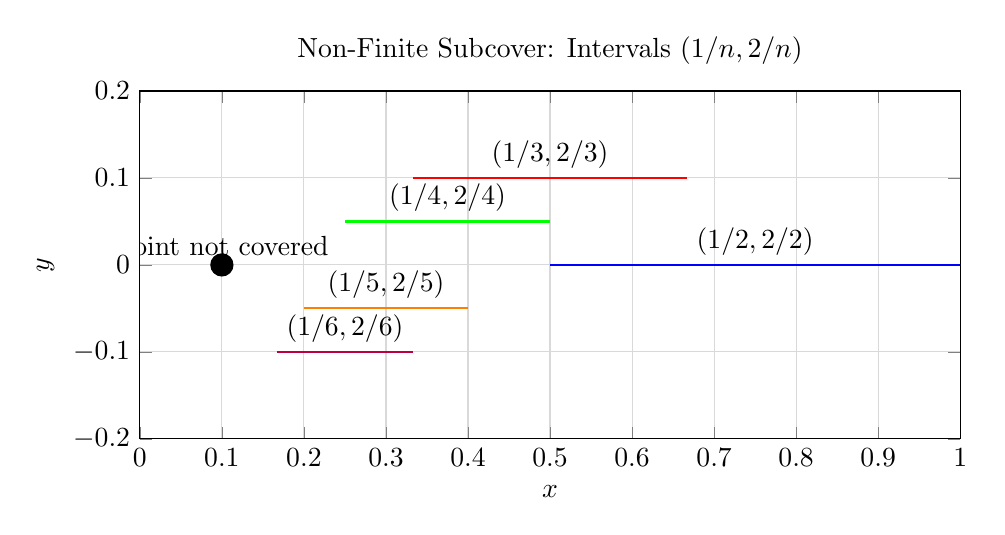
\begin{tikzpicture}
\begin{axis}[
    width=12cm,
    height=6cm,
    xlabel={$x$},
    ylabel={$y$},
    title={Non-Finite Subcover: Intervals $(1/n, 2/n)$},
    xmin=0, xmax=1,
    ymin=-0.2, ymax=0.2,
    grid=major,
    grid style={gray!30},
    legend pos=north east
]

% Several intervals
\addplot[blue, thick] coordinates {(0.5,0) (1,0)};
\addplot[red, thick] coordinates {(0.333,0.1) (0.667,0.1)};
\addplot[green, thick] coordinates {(0.25,0.05) (0.5,0.05)};
\addplot[orange, thick] coordinates {(0.2,-0.05) (0.4,-0.05)};
\addplot[purple, thick] coordinates {(0.167,-0.1) (0.333,-0.1)};

% Labels
\node[above] at (axis cs:0.75,0) {$(1/2, 2/2)$};
\node[above] at (axis cs:0.5,0.1) {$(1/3, 2/3)$};
\node[above] at (axis cs:0.375,0.05) {$(1/4, 2/4)$};
\node[above] at (axis cs:0.3,-0.05) {$(1/5, 2/5)$};
\node[above] at (axis cs:0.25,-0.1) {$(1/6, 2/6)$};

% Point not covered by finite subcollection
\addplot[black, mark=*, mark size=4pt] coordinates {(0.1,0)};
\node[above] at (axis cs:0.1,0) {Point not covered};

\end{axis}
\end{tikzpicture}
\caption{The collection of intervals $(1/n, 2/n)$ covers $(0,1)$ but no finite subcollection covers it. The point $0.1$ is not covered by any interval in a finite subcollection.}
\end{figure}

\bigskip\noindent\textbf{Solution:} Let $\mathcal{G} = \{(1/n_1, 2/n_1), \ldots, (1/n_k, 2/n_k)\}$ be a finite subcollection of $\mathcal{F}$. Let $N = \max\{n_1, \ldots, n_k\}$.

Then the leftmost interval in $\mathcal{G}$ is $(1/N, 2/N)$. For any $x \in (0, 1/N)$, we have $x < 1/N < 2/N$, so $x$ is not covered by any interval in $\mathcal{G}$.

Therefore, $\mathcal{G}$ does not cover $(0,1)$, proving that no finite subcollection of $\mathcal{F}$ covers $(0,1)$.\qed


\begin{problembox}[3.20: Closed but Not Bounded Set with Infinite Covering]
\begin{problemstatement}
Give an example of a set \( S \) which is closed but not bounded and exhibit a countable open covering \( \mathcal{F} \) such that no finite subset of \( \mathcal{F} \) covers \( S \).
\end{problemstatement}
\end{problembox}

\noindent\textbf{Strategy:} Use the integers $\mathbb{Z}$ as the set (closed but not bounded). Create a covering where each integer has its own interval, making it impossible for any finite subcollection to cover the infinite set.

% Visualization for Exercise 3.20: Closed but Not Bounded Set
\begin{figure}[h]
\centering
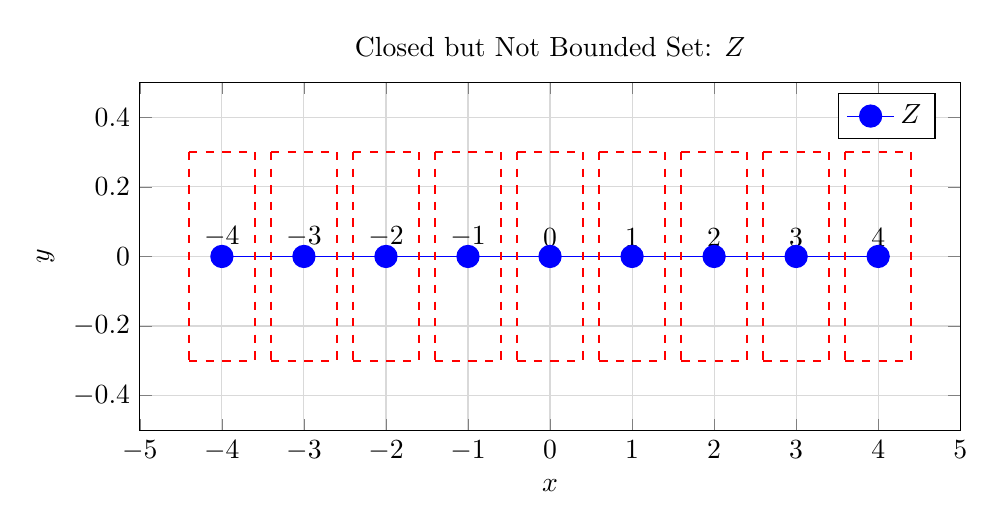
\begin{tikzpicture}
\begin{axis}[
    width=12cm,
    height=6cm,
    xlabel={$x$},
    ylabel={$y$},
    title={Closed but Not Bounded Set: $\mathbb{Z}$},
    xmin=-5, xmax=5,
    ymin=-0.5, ymax=0.5,
    grid=major,
    grid style={gray!30},
    legend pos=north east
]

% Integer points
\addplot[blue, mark=*, mark size=4pt] coordinates {
    (-4,0) (-3,0) (-2,0) (-1,0) (0,0) (1,0) (2,0) (3,0) (4,0)
};
\addlegendentry{$\mathbb{Z}$}

% Neighborhoods around each integer
\foreach \x in {-4,-3,-2,-1,0,1,2,3,4} {
    \addplot[red, dashed, thick] coordinates {(\x-0.4,0.3) (\x+0.4,0.3)};
    \addplot[red, dashed, thick] coordinates {(\x-0.4,-0.3) (\x+0.4,-0.3)};
    \addplot[red, dashed, thick] coordinates {(\x-0.4,0.3) (\x-0.4,-0.3)};
    \addplot[red, dashed, thick] coordinates {(\x+0.4,0.3) (\x+0.4,-0.3)};
}

% Labels
\node[above] at (axis cs:-4,0) {$-4$};
\node[above] at (axis cs:-3,0) {$-3$};
\node[above] at (axis cs:-2,0) {$-2$};
\node[above] at (axis cs:-1,0) {$-1$};
\node[above] at (axis cs:0,0) {$0$};
\node[above] at (axis cs:1,0) {$1$};
\node[above] at (axis cs:2,0) {$2$};
\node[above] at (axis cs:3,0) {$3$};
\node[above] at (axis cs:4,0) {$4$};

\end{axis}
\end{tikzpicture}
\caption{The set of integers $\mathbb{Z}$ is closed but not bounded. Each integer has a neighborhood that contains no other integers, showing it has no accumulation points.}
\end{figure}

\bigskip\noindent\textbf{Solution:} Let $S = \mathbb{Z}$ (the set of integers). This set is closed but not bounded.

Let $\mathcal{F} = \{(n-1/2, n+1/2) : n \in \mathbb{Z}\}$. This is a countable open covering of $\mathbb{Z}$ since each integer $n$ is contained in the interval $(n-1/2, n+1/2)$.

However, no finite subcollection of $\mathcal{F}$ covers $\mathbb{Z}$. If $\mathcal{G} = \{(n_1-1/2, n_1+1/2), \ldots, (n_k-1/2, n_k+1/2)\}$ is a finite subcollection, then $\mathcal{G}$ can only cover finitely many integers, but $\mathbb{Z}$ is infinite.

Therefore, $\mathcal{F}$ is a countable open covering of $S$ with no finite subcover.\qed


\begin{problembox}[3.21: Countability via Local Countability]
\begin{problemstatement}
Given a set \( S \) in \( \mathbb{R}^n \) with the property that for every \( x \) in \( S \) there is an \( n \)-ball \( B(x) \) such that \( B(x) \cap S \) is countable. Prove that \( S \) is countable.
\end{problemstatement}
\end{problembox}

\noindent\textbf{Strategy:} Use the Lindelöf property of $\mathbb{R}^n$ (every open cover has a countable subcover). The collection of balls $\{B(x) : x \in S\}$ covers $S$, so there's a countable subcover. Each ball in the subcover intersects $S$ in a countable set, so $S$ is a countable union of countable sets.

\bigskip\noindent\textbf{Solution:}\\
For each point $\mathbf{x} \in S$, we are given that there exists an open ball $B_\mathbf{x}$ centered at $\mathbf{x}$ such that the set $B_\mathbf{x} \cap S$ is countable.

The collection of all such balls, $\mathcal{C} = \{B_\mathbf{x} : \mathbf{x} \in S\}$, forms an open covering of the set $S$ (since each $\mathbf{x} \in S$ is in its own ball $B_\mathbf{x}$).

The space $\mathbb{R}^n$ is a \textbf{separable} metric space because it contains a countable dense subset, $\mathbb{Q}^n$. A key theorem in topology states that every separable metric space has the \textbf{Lindelöf property}. This property guarantees that any open covering of a set in that space has a countable subcovering.

Applying the Lindelöf property to our open cover $\mathcal{C}$ of $S$, we can extract a countable subcollection, say $\mathcal{C}' = \{B_{\mathbf{x}_k} : k \in \mathbb{N}\}$, that still covers $S$. This means:
$$S \subseteq \bigcup_{k=1}^{\infty} B_{\mathbf{x}_k}$$
From this, we can express the set $S$ as:
$$S = S \cap \left( \bigcup_{k=1}^{\infty} B_{\mathbf{x}_k} \right) = \bigcup_{k=1}^{\infty} (S \cap B_{\mathbf{x}_k})$$
By the initial hypothesis, each set in this union, $(S \cap B_{\mathbf{x}_k})$, is countable.
Therefore, $S$ is a countable union of countable sets. A fundamental result of set theory states that a countable union of countable sets is itself countable. Thus, we conclude that the set $S$ must be countable.\qed


\begin{problembox}[3.22: Countability of Disjoint Open Sets]
\begin{problemstatement}
Prove that a collection of disjoint open sets in \( \mathbb{R}^n \) is necessarily countable. Give an example of a collection of disjoint closed sets which is not countable.
\end{problemstatement}
\end{problembox}

\noindent\textbf{Strategy:} Use the separability of $\mathbb{R}^n$ - each open set contains a point from the countable dense subset, and since the sets are disjoint, each dense point can belong to at most one set. For the counterexample, use singletons of real numbers.

\bigskip\noindent\textbf{Solution:} Let $\mathcal{F}$ be a collection of disjoint open sets in $\mathbb{R}^n$. Since $\mathbb{R}^n$ is separable, there exists a countable dense subset $D$.

For each open set $U \in \mathcal{F}$, there exists a point $d \in D$ such that $d \in U$. Since the sets in $\mathcal{F}$ are disjoint, each point $d \in D$ can belong to at most one set in $\mathcal{F}$.

Therefore, the number of sets in $\mathcal{F}$ is at most the number of points in $D$, which is countable.

For an example of uncountably many disjoint closed sets, let $\mathcal{G} = \{\{x\} : x \in \mathbb{R}\}$. Each singleton $\{x\}$ is closed, the sets are disjoint, and there are uncountably many real numbers.\qed


\begin{problembox}[3.23: Existence of Condensation Points]
\begin{problemstatement}
Assume that \( S \subseteq \mathbb{R}^n \). A point \( x \) in \( \mathbb{R}^n \) is said to be a condensation point of \( S \) if every \( n \)-ball \( B(x) \) has the property that \( B(x) \cap S \) is not countable. Prove that if \( S \) is not countable, then there exists a point \( x \) in \( S \) such that \( x \) is a condensation point of \( S \).
\end{problemstatement}
\end{problembox}

\noindent\textbf{Strategy:} Use proof by contradiction. If no point is a condensation point, then every point has a neighborhood where the intersection with $S$ is countable. Apply Exercise 3.21 to conclude that $S$ is countable, contradicting the hypothesis.

\bigskip\noindent\textbf{Solution:} Suppose for contradiction that no point in $S$ is a condensation point of $S$. Then for every $x \in S$, there exists an $n$-ball $B_x$ centered at $x$ such that $B_x \cap S$ is countable.

By Exercise 3.21, this implies that $S$ is countable, which contradicts the hypothesis that $S$ is not countable.

Therefore, there must exist at least one point $x \in S$ that is a condensation point of $S$.\qed


\begin{problembox}[3.24: Properties of Condensation Points]
\begin{problemstatement}
Assume that \( S \subseteq \mathbb{R}^n \) and that \( S \) is not countable. Let \( T \) denote the set of condensation points of \( S \). Prove that:
\begin{enumerate}[label=\alph*)]
\item \( S - T \) is countable,
\item \( S \cap T \) is not countable,
\item \( T \) is closed,
\item \( T \) contains no isolated points.
\end{enumerate}
Note that Exercise 3.23 is a special case of (b).
\end{problemstatement}
\end{problembox}

\noindent\textbf{Strategy:} For (a), use Exercise 3.21. For (b), use the fact that $S$ is uncountable and $S-T$ is countable. For (c), show that if a point is in the closure of $T$, it's a condensation point. For (d), use the fact that $S-T$ is countable and any neighborhood of a condensation point contains uncountably many points of $S$.

\bigskip\noindent\textbf{Solution:} 
(a) For each $x \in S - T$, there exists an $n$-ball $B_x$ centered at $x$ such that $B_x \cap S$ is countable. By Exercise 3.21, $S - T$ is countable.

(b) Since $S$ is not countable and $S - T$ is countable, $S \cap T$ must be uncountable.

(c) Let $x \in \overline{T}$. Then every neighborhood of $x$ contains a point of $T$. Let $B$ be any $n$-ball centered at $x$. There exists $y \in T \cap B$. Since $y$ is a condensation point, $B(y;r) \cap S$ is uncountable for any $r > 0$. Choose $r$ small enough so that $B(y;r) \subset B$. Then $B \cap S$ contains the uncountable set $B(y;r) \cap S$, so $x$ is a condensation point. Therefore, $T$ is closed.

(d) Let $x \in T$. For any $\varepsilon > 0$, $B(x;\varepsilon) \cap S$ is uncountable. Since $S - T$ is countable, $B(x;\varepsilon) \cap T$ must be uncountable. Therefore, $x$ is not isolated in $T$.\qed


\begin{problembox}[3.25: Cantor-Bendixon Theorem]
\begin{problemstatement}
A set in \( \mathbb{R}^n \) is called perfect if \( S = S' \), that is, if \( S \) is a closed set which contains no isolated points. Prove that every uncountable closed set \( F \) in \( \mathbb{R}^n \) can be expressed in the form \( F = A \cup B \), where \( A \) is perfect and \( B \) is countable (Cantor-Bendixon theorem).

\textit{Hint.} Use Exercise 3.24.
\end{problemstatement}
\end{problembox}

\noindent\textbf{Strategy:} Use Exercise 3.24 to take $A$ as the set of condensation points $T$ and $B$ as $F-T$. Show that $T$ is perfect (closed with no isolated points) and $F-T$ is countable.

\bigskip\noindent\textbf{Solution:} Let $F$ be an uncountable closed set in $\mathbb{R}^n$. Let $T$ be the set of condensation points of $F$. By Exercise 3.24, $T$ is closed and $F - T$ is countable.

Let $A = T$ and $B = F - T$. Then $F = A \cup B$ where $B$ is countable.

We need to show that $A$ is perfect. Since $T$ is closed by Exercise 3.24(c), $A$ is closed. By Exercise 3.24(d), $T$ contains no isolated points, so $A$ contains no isolated points.

Therefore, $A$ is perfect, and we have the desired decomposition $F = A \cup B$.\qed
\section{Metric Spaces}

\subsection*{Definitions and Theorems for Section 3.4}

\begin{definition}[Metric Space]
A metric space consists of a set $M$ together with a function $d: M \times M \to [0,\infty)$ (called a metric or distance function) that satisfies the following three axioms for all points $x, y, z \in M$:
\begin{enumerate}
\item $d(x,y) = 0$ if and only if $x = y$ (positive definiteness)
\item $d(x,y) = d(y,x)$ for all $x,y \in M$ (symmetry)
\item $d(x,z) \leq d(x,y) + d(y,z)$ for all $x,y,z \in M$ (triangle inequality)
\end{enumerate}
\end{definition}

\begin{definition}[Closed Ball]
Given a metric space $(M,d)$, the closed ball centered at a point $a \in M$ with radius $r > 0$ is the set $\overline{B}(a;r) = \{x \in M : d(x,a) \leq r\}$.
\end{definition}

\begin{theorem}[Separability of Euclidean Spaces]
Every Euclidean space $\mathbb{R}^n$ is separable.
\end{theorem}

\begin{theorem}[Bounded Metric Construction]
If $(M,d)$ is a metric space, then the function $d'(x,y) = \frac{d(x,y)}{1 + d(x,y)}$ defines a metric on $M$ that is bounded above by 1.
\end{theorem}

\begin{theorem}[Product Metrics]
Given two metric spaces $(S_1,d_1)$ and $(S_2,d_2)$, the following functions define metrics on the Cartesian product $S_1 \times S_2$:
\begin{enumerate}
\item $\rho(x,y) = d_1(x_1,y_1) + d_2(x_2,y_2)$ (sum metric)
\item $\rho(x,y) = \max\{d_1(x_1,y_1), d_2(x_2,y_2)\}$ (maximum metric)
\item $\rho(x,y) = \sqrt{d_1(x_1,y_1)^2 + d_2(x_2,y_2)^2}$ (Euclidean product metric)
\end{enumerate}
\end{theorem}

\begin{theorem}[Finite Sets are Closed]
Every finite subset of a metric space is a closed set.
\end{theorem}

\begin{theorem}[Closed Balls are Closed]
In any metric space, every closed ball is a closed set.
\end{theorem}

\begin{theorem}[Transitivity of Density]
If $A$ is dense in $S$ and $S$ is dense in $T$, then $A$ is dense in $T$.
\end{theorem}

\begin{theorem}[Density and Open Sets]
If $A$ is dense in $S$ and $B$ is an open subset of $S$, then $B$ is contained in the closure of $A \cap B$.
\end{theorem}

\begin{theorem}[Intersection of Dense and Open Sets]
If both $A$ and $B$ are dense in $S$ and $B$ is an open subset of $S$, then the intersection $A \cap B$ is dense in $S$.
\end{theorem}



\begin{problembox}[3.26: Open and Closed Sets in Metric Spaces]
\begin{problemstatement}
In any metric space \((M, d)\), prove that the empty set \( \emptyset \) and the whole space \( M \) are both open and closed.
\end{problemstatement}
\end{problembox}

\noindent\textbf{Strategy:} Use the definitions of open and closed sets directly. For the empty set, use vacuous truth for openness and complementarity for closedness. For the whole space, use the definition of open balls and complementarity.

\noindent\bigskip\noindent\textbf{Solution:} The empty set $\emptyset$ is open because the condition "for every point in $\emptyset$, there exists a neighborhood contained in $\emptyset$" is vacuously true (there are no points to check).

The empty set $\emptyset$ is closed because its complement $M$ is open.

The whole space $M$ is open because for any point $x \in M$ and any $\varepsilon > 0$, the ball $B(x;\varepsilon) \subset M$.

The whole space $M$ is closed because its complement $\emptyset$ is open.\qed


\begin{problembox}[3.27: Metric Balls in Different Metrics]
\begin{problemstatement}
Consider the following two metrics in \( \mathbb{R}^n \):
\[d_1(x, y) = \max_{1 \leq i \leq n} |x_i - y_i|, \quad d_2(x, y) = \sum_{i=1}^n |x_i - y_i|.\]

In each of the following metric spaces prove that the ball \( B(a; r) \) has the geometric appearance indicated:
\begin{enumerate}[label=\alph*)]
\item In \( (\mathbb{R}^2, d_1) \), a square with sides parallel to the coordinate axes.
\item In \( (\mathbb{R}^2, d_2) \), a square with diagonals parallel to the axes.
\item A cube in \( (\mathbb{R}^3, d_1) \).
\item An octahedron in \( (\mathbb{R}^3, d_2) \).
\end{enumerate}
\end{problemstatement}
\end{problembox}

\noindent\textbf{Strategy:} Use the definition of metric balls $B(a;r) = \{x : d(a,x) < r\}$ and substitute the given metrics. For $d_1$, the maximum constraint creates axis-aligned shapes. For $d_2$, the sum constraint creates diamond/octahedral shapes.

% Visualization for Exercise 3.27: Metric Balls
\begin{figure}[h]
\centering
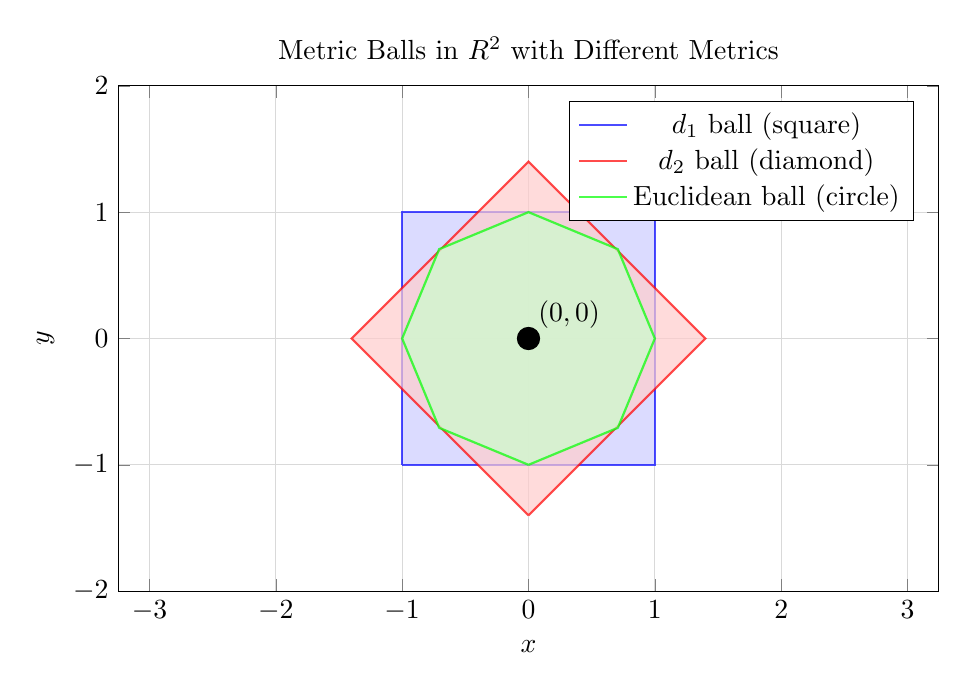
\begin{tikzpicture}
\begin{axis}[
    width=12cm,
    height=8cm,
    xlabel={$x$},
    ylabel={$y$},
    title={Metric Balls in $\mathbb{R}^2$ with Different Metrics},
    xmin=-2, xmax=2,
    ymin=-2, ymax=2,
    grid=major,
    grid style={gray!30},
    legend pos=north east,
    axis equal
]

% d_1 metric ball (square)
\addplot[blue, thick, fill=blue!20, opacity=0.7] coordinates {
    (-1,-1) (1,-1) (1,1) (-1,1) (-1,-1)
};
\addlegendentry{$d_1$ ball (square)}

% d_2 metric ball (diamond)
\addplot[red, thick, fill=red!20, opacity=0.7] coordinates {
    (0,-1.4) (1.4,0) (0,1.4) (-1.4,0) (0,-1.4)
};
\addlegendentry{$d_2$ ball (diamond)}

% Euclidean ball (circle)
\addplot[green, thick, fill=green!20, opacity=0.7] coordinates {
    (0,-1) (0.707,-0.707) (1,0) (0.707,0.707) (0,1) (-0.707,0.707) (-1,0) (-0.707,-0.707) (0,-1)
};
\addlegendentry{Euclidean ball (circle)}

% Center point
\addplot[black, mark=*, mark size=4pt] coordinates {(0,0)};
\node[above right] at (axis cs:0,0) {$(0,0)$};

\end{axis}
\end{tikzpicture}
\caption{Comparison of metric balls centered at $(0,0)$ with radius 1: $d_1$ produces a square, $d_2$ produces a diamond, and the Euclidean metric produces a circle.}
\end{figure}

\bigskip\noindent\textbf{Solution:} 
(a) In $(\mathbb{R}^2, d_1)$, the ball $B(a;r) = \{(x,y) : \max\{|x-a_1|, |y-a_2|\} < r\}$. This means $|x-a_1| < r$ and $|y-a_2| < r$, which defines a square with center $(a_1,a_2)$ and sides of length $2r$ parallel to the coordinate axes.

(b) In $(\mathbb{R}^2, d_2)$, the ball $B(a;r) = \{(x,y) : |x-a_1| + |y-a_2| < r\}$. This defines a diamond-shaped region (square rotated 45 degrees) with diagonals parallel to the axes.

(c) In $(\mathbb{R}^3, d_1)$, the ball $B(a;r) = \{(x,y,z) : \max\{|x-a_1|, |y-a_2|, |z-a_3|\} < r\}$. This defines a cube with center $(a_1,a_2,a_3)$ and sides of length $2r$ parallel to the coordinate axes.

(d) In $(\mathbb{R}^3, d_2)$, the ball $B(a;r) = \{(x,y,z) : |x-a_1| + |y-a_2| + |z-a_3| < r\}$. This defines an octahedron with center $(a_1,a_2,a_3)$.\qed


\begin{problembox}[3.28: Metric Inequalities]
\begin{problemstatement}
Let \( d_1 \) and \( d_2 \) be the metrics of Exercise 3.27 and let \( \|x - y\| \) denote the usual Euclidean metric. Prove the following inequalities for all \( x \) and \( y \) in \( \mathbb{R}^n \):
\[d_1(x, y) \leq \|x - y\| \leq d_2(x, y) \quad \text{and} \quad d_2(x, y) \leq \sqrt{n} \|x - y\| \leq n\,d_1(x, y).\]
\end{problemstatement}
\end{problembox}

\noindent\textbf{Strategy:} Use the definitions of the metrics and basic inequalities. For the first part, use the fact that the maximum is less than or equal to the square root of the sum of squares, and the square root is less than or equal to the sum. For the second part, use the Cauchy-Schwarz inequality.

\bigskip\noindent\textbf{Solution:} Let $x, y \in \mathbb{R}^n$. Let $a_i = |x_i - y_i|$ for $1 \leq i \leq n$. Then:

(1) \( d_1(x, y) = \max_i a_i \leq \sqrt{\sum a_i^2} = \|x - y\| \) (since each $a_i^2 \leq \sum a_i^2$)

(2) \( \|x - y\| = \sqrt{\sum a_i^2} \leq \sum a_i = d_2(x,y) \) (by the inequality \( \sqrt{a_1^2 + \dots + a_n^2} \leq a_1 + \dots + a_n \))

(3) By the Cauchy-Schwarz inequality:
\[
\left(\sum a_i\right)^2 \leq n \sum a_i^2 \Rightarrow d_2(x,y) \leq \sqrt{n} \|x - y\|
\]

(4) Also, since \( \|x - y\| = \sqrt{\sum a_i^2} \leq \sqrt{n \cdot \max_i a_i^2} = \sqrt{n} \cdot \max a_i = \sqrt{n} d_1(x, y) \), it follows that:

\[
\sqrt{n} \|x - y\| \leq n d_1(x, y)
\]

Hence, all inequalities hold:

\[
d_1(x,y) \leq \|x - y\| \leq d_2(x,y), \quad d_2(x, y) \leq \sqrt{n} \|x - y\| \leq n\,d_1(x, y)
\]\qed


\begin{problembox}[3.29: Bounded Metric]
\begin{problemstatement}
If \( (M, d) \) is a metric space, define
\[d'(x, y) = \frac{d(x, y)}{1 + d(x, y)}.\]
Prove that \( d' \) is also a metric for \( M \). Note that \( 0 \leq d'(x, y) < 1 \) for all \( x, y \) in \( M \).
\end{problemstatement}
\end{problembox}

\noindent\textbf{Strategy:} Verify the three metric properties: non-negativity, symmetry, and triangle inequality. For the triangle inequality, use the fact that the function $f(t) = t/(1+t)$ is increasing and the inequality $\frac{a+b}{1+a+b} \leq \frac{a}{1+a} + \frac{b}{1+b}$ for non-negative $a,b$.

\bigskip\noindent\textbf{Solution:} We need to verify the three properties of a metric:

(1) $d'(x,y) \geq 0$ since $d(x,y) \geq 0$ and $1 + d(x,y) > 0$.

(2) $d'(x,y) = 0$ if and only if $d(x,y) = 0$, which occurs if and only if $x = y$.

(3) $d'(x,y) = d'(y,x)$ since $d(x,y) = d(y,x)$.

(4) For the triangle inequality, let $f(t) = \frac{t}{1+t}$. Then $f'(t) = \frac{1}{(1+t)^2} > 0$, so $f$ is increasing. Therefore, $d'(x,z) = f(d(x,z)) \leq f(d(x,y) + d(y,z)) = \frac{d(x,y) + d(y,z)}{1 + d(x,y) + d(y,z)} \leq \frac{d(x,y)}{1 + d(x,y)} + \frac{d(y,z)}{1 + d(y,z)} = d'(x,y) + d'(y,z)$.

The last inequality follows from the fact that $\frac{a+b}{1+a+b} \leq \frac{a}{1+a} + \frac{b}{1+b}$ for $a,b \geq 0$.\qed


\begin{problembox}[3.30: Finite Sets in Metric Spaces]
\begin{problemstatement}
Prove that every finite subset of a metric space is closed.
\end{problemstatement}
\end{problembox}

\noindent\textbf{Strategy:} Show that the complement is open. For any point not in the finite set, find a minimum distance to the set and use that to construct a neighborhood that doesn't intersect the set.

\bigskip\noindent\textbf{Solution:} Let $S = \{x_1, x_2, \ldots, x_n\}$ be a finite subset of a metric space $(M,d)$. We need to show that the complement $M \setminus S$ is open.

Let $x \in M \setminus S$. Let $\varepsilon = \min\{d(x,x_i) : i = 1,2,\ldots,n\}$. Since $x \notin S$, we have $\varepsilon > 0$.

Then $B(x;\varepsilon) \cap S = \emptyset$, so $B(x;\varepsilon) \subset M \setminus S$. This shows that every point in $M \setminus S$ is an interior point, so $M \setminus S$ is open.

Therefore, $S$ is closed.\qed


\begin{problembox}[3.31: Closed Balls in Metric Spaces]
\begin{problemstatement}
In a metric space \((M, d)\) the closed ball of radius \( r > 0 \) about a point \( a \) in \( M \) is the set \( \overline{B}(a; r) = \{x : d(x, a) \leq r\} \).
\begin{enumerate}[label=\alph*)]
\item Prove that \( \overline{B}(a; r) \) is a closed set.
\item Give an example of a metric space in which \( \overline{B}(a; r) \) is not the closure of the open ball \( B(a; r) \).
\end{enumerate}
\end{problemstatement}
\end{problembox}

\noindent\textbf{Strategy:} For (a), show the complement is open by using the triangle inequality to find a neighborhood around any point outside the closed ball. For (b), use a discrete metric space where the open ball is a singleton but the closed ball is the entire space.

\bigskip\noindent\textbf{Solution:} 
(a) Let $x \in M \setminus \overline{B}(a;r)$. Then $d(x,a) > r$. Let $\varepsilon = d(x,a) - r > 0$. For any $y \in B(x;\varepsilon)$, we have $d(y,a) \geq d(x,a) - d(x,y) > d(x,a) - \varepsilon = r$. Therefore, $B(x;\varepsilon) \subset M \setminus \overline{B}(a;r)$, showing that $M \setminus \overline{B}(a;r)$ is open. Hence, $\overline{B}(a;r)$ is closed.

(b) Consider the discrete metric space $(M,d)$ where $d(x,y) = 1$ if $x \neq y$ and $d(x,y) = 0$ if $x = y$. Let $a \in M$ and $r = 1$. Then $B(a;1) = \{a\}$ and $\overline{B}(a;1) = M$. The closure of $B(a;1)$ is $\{a\}$, which is not equal to $\overline{B}(a;1) = M$.\qed


\begin{problembox}[3.32: Transitivity of Density]
\begin{problemstatement}
In a metric space \( M \), if subsets satisfy \( A \subseteq S \subseteq \overline{A} \), where \(\overline{A}\) is the closure of \( A \), then \( A \) is said to be dense in \( S \). For example, the set \( \mathbb{Q} \) of rational numbers is dense in \( \mathbb{R} \). If \( A \) is dense in \( S \) and if \( S \) is dense in \( T \), prove that \( A \) is dense in \( T \).
\end{problemstatement}
\end{problembox}

\noindent\textbf{Strategy:} Use the definition of density and the fact that closure is idempotent ($\overline{\overline{A}} = \overline{A}$). Show that $A \subseteq T \subseteq \overline{A}$ by using the density relationships and the transitivity of subset inclusion.

\bigskip\noindent\textbf{Solution:} We need to show that $A \subseteq T \subseteq \overline{A}$.

Since $A \subseteq S \subseteq T$, we have $A \subseteq T$.

Since $S$ is dense in $T$, we have $T \subseteq \overline{S}$. Since $A$ is dense in $S$, we have $S \subseteq \overline{A}$. Therefore, $\overline{S} \subseteq \overline{\overline{A}} = \overline{A}$.

Combining these, we get $T \subseteq \overline{S} \subseteq \overline{A}$, so $T \subseteq \overline{A}$.

Therefore, $A \subseteq T \subseteq \overline{A}$, showing that $A$ is dense in $T$.\qed


\begin{problembox}[3.33: Separability of Euclidean Spaces]
\begin{problemstatement}
A metric space \( M \) is said to be separable if there is a countable subset \( A \) which is dense in \( M \). For example, \( \mathbb{R} \) is separable because the set \( \mathbb{Q} \) of rational numbers is a countable dense subset. Prove that every Euclidean space \( \mathbb{R}^k \) is separable.
\end{problemstatement}
\end{problembox}

\noindent\textbf{Strategy:} Use the Cartesian product of rational numbers $\mathbb{Q}^k$ as the countable dense subset. Show it's countable (product of countable sets) and dense (use the density of rationals in each coordinate and the triangle inequality).

\bigskip\noindent\textbf{Solution:} Let $A$ be the set of all points in $\mathbb{R}^k$ with rational coordinates. That is, $A = \{(q_1, q_2, \ldots, q_k) : q_i \in \mathbb{Q} \text{ for } i = 1,2,\ldots,k\}$.

Since $\mathbb{Q}$ is countable, the Cartesian product $A = \mathbb{Q}^k$ is countable.

To show that $A$ is dense in $\mathbb{R}^k$, let $x = (x_1, x_2, \ldots, x_k) \in \mathbb{R}^k$ and $\varepsilon > 0$. Since $\mathbb{Q}$ is dense in $\mathbb{R}$, for each $i$ there exists $q_i \in \mathbb{Q}$ such that $|x_i - q_i| < \varepsilon/\sqrt{k}$.

Then $q = (q_1, q_2, \ldots, q_k) \in A$ and $\|x - q\| = \sqrt{\sum_{i=1}^k (x_i - q_i)^2} < \sqrt{k(\varepsilon/\sqrt{k})^2} = \varepsilon$.

Therefore, $A$ is a countable dense subset of $\mathbb{R}^k$, so $\mathbb{R}^k$ is separable.\qed


\begin{problembox}[3.34: Lindelöf Theorem in Separable Spaces]
\begin{problemstatement}
Prove that the Lindelöf covering theorem (Theorem 3.28) is valid in any separable metric space.
\end{problemstatement}
\end{problembox}

\noindent\textbf{Strategy:} Use the countable dense subset to construct a countable subcover. For each point in the dense subset, choose a set from the open cover that contains it, and show that this countable collection covers the entire space.

\bigskip\noindent\textbf{Solution:} Let $M$ be a separable metric space with countable dense subset $D = \{d_1, d_2, \ldots\}$. Let $\mathcal{F}$ be an open covering of $M$.

For each $d_i \in D$ and each positive rational $r$, if there exists a set $F \in \mathcal{F}$ such that $B(d_i;r) \subset F$, let $F_{i,r}$ be one such set.

The collection $\{F_{i,r} : i \in \mathbb{N}, r \in \mathbb{Q}^+, B(d_i;r) \subset F_{i,r} \text{ for some } F \in \mathcal{F}\}$ is countable.

We claim this collection covers $M$. Let $x \in M$. Since $\mathcal{F}$ covers $M$, there exists $F \in \mathcal{F}$ such that $x \in F$. Since $F$ is open, there exists $\varepsilon > 0$ such that $B(x;\varepsilon) \subset F$.

Since $D$ is dense, there exists $d_i \in D$ such that $d_i \in B(x;\varepsilon/2)$. Let $r$ be a rational number such that $d(x,d_i) < r < \varepsilon/2$. Then $B(d_i;r) \subset B(x;\varepsilon) \subset F$.

Therefore, $F_{i,r}$ exists and contains $x$, showing that the countable subcollection covers $M$.\qed


\begin{problembox}[3.35: Density and Open Sets]
\begin{problemstatement}
If \( A \) is dense in \( S \) and if \( B \) is open in \( S \), prove that \( B \subseteq \overline{A \cap B} \).

\textit{Hint.} Exercise 3.13.
\end{problemstatement}
\end{problembox}

\noindent\textbf{Strategy:} Use the definition of density and the fact that $B$ is open. For any point $x \in B$, show that any neighborhood of $x$ contains a point from $A \cap B$ by using the density of $A$ and the openness of $B$.

\bigskip\noindent\textbf{Solution:}\\
The statement "$A$ is dense in $S$" means $S \subseteq \overline{A}$. We are given that $A \subseteq S$.
The statement "$B$ is open in $S$" means that $B = V \cap S$ for some set $V$ that is open in the larger metric space $M$.

Let $x \in B$. We want to show that $x \in \overline{A \cap B}$. This requires showing that any open neighborhood of $x$ in $M$ has a non-empty intersection with the set $A \cap B$.

Let $U$ be an arbitrary open neighborhood of $x$ in $M$.
Since $x \in B$ and $B = V \cap S$, we have $x \in V$.
The set $U \cap V$ is also an open neighborhood of $x$ because it is the intersection of two open sets.

Since $x \in B \subseteq S$ and $A$ is dense in $S$, $x$ is an adherent point of $A$. Therefore, the open neighborhood $U \cap V$ must contain a point from $A$. Let's call this point $y$.
So, $y \in (U \cap V) \cap A$.

Now we check if this point $y$ is in the required sets:
\begin{itemize}
    \item $y \in U$, so $y$ is in the arbitrary neighborhood of $x$.
    \item $y \in A$.
    \item We need to show $y \in B$. We know $y \in V$. Since we are given $A \subseteq S$, and $y \in A$, it follows that $y \in S$.
\end{itemize}
Since $y \in V$ and $y \in S$, we have $y \in V \cap S$, which means $y \in B$.

So we have found a point $y$ such that $y \in U$ and $y \in A \cap B$. This means $U \cap (A \cap B) \neq \emptyset$.
Since $U$ was an arbitrary open neighborhood of $x$, this proves that $x \in \overline{A \cap B}$.
As this holds for any $x \in B$, we conclude that $B \subseteq \overline{A \cap B}$.\qed


\begin{problembox}[3.36: Intersection of Dense and Open Sets]
\begin{problemstatement}
If each of \( A \) and \( B \) is dense in \( S \) and if \( B \) is open in \( S \), prove that \( A \cap B \) is dense in \( S \).
\end{problemstatement}
\end{problembox}

\noindent\textbf{Strategy:} Use the fact that $B$ is open to find a neighborhood around any point in $S$ that is contained in $B$. Then use the density of $A$ to find a point in that neighborhood that belongs to both $A$ and $B$.

\bigskip\noindent\textbf{Solution:} We need to show that $S \subseteq \overline{A \cap B}$.

Let $x \in S$. Since $B$ is open in $S$, there exists $\varepsilon > 0$ such that $B(x;\varepsilon) \cap S \subset B$.

Since $A$ is dense in $S$, $B(x;\varepsilon) \cap A \neq \emptyset$. Let $y \in B(x;\varepsilon) \cap A$. Since $y \in S$ and $B(x;\varepsilon) \cap S \subset B$, we have $y \in B$.

Therefore, $y \in A \cap B$, so $B(x;\varepsilon) \cap (A \cap B) \neq \emptyset$.

This shows that every neighborhood of $x$ contains a point of $A \cap B$, so $x \in \overline{A \cap B}$.

Therefore, $S \subseteq \overline{A \cap B}$, showing that $A \cap B$ is dense in $S$.\qed


\begin{problembox}[3.37: Product Metrics]
\begin{problemstatement}
Given two metric spaces \((S_1, d_1)\) and \((S_2, d_2)\), a metric \( \rho \) for the Cartesian product \( S_1 \times S_2 \) can be constructed from \( d_1 \) and \( d_2 \) in many ways. For example, if \( x = (x_1, x_2) \) and \( y = (y_1, y_2) \) are in \( S_1 \times S_2 \), let \( \rho(x, y) = d_1(x_1, y_1) + d_2(x_2, y_2) \). Prove that \( \rho \) is a metric for \( S_1 \times S_2 \) and construct further examples.
\end{problemstatement}
\end{problembox}

\noindent\textbf{Strategy:} Verify the three metric properties for the sum metric. For the triangle inequality, use the triangle inequalities of the individual metrics. For additional examples, consider maximum, Euclidean, and $p$-norms.

\bigskip\noindent\textbf{Solution:} We need to verify the three properties of a metric for $\rho(x,y) = d_1(x_1,y_1) + d_2(x_2,y_2)$:

(1) $\rho(x,y) \geq 0$ since $d_1(x_1,y_1) \geq 0$ and $d_2(x_2,y_2) \geq 0$.

(2) $\rho(x,y) = 0$ if and only if $d_1(x_1,y_1) = 0$ and $d_2(x_2,y_2) = 0$, which occurs if and only if $x_1 = y_1$ and $x_2 = y_2$, i.e., $x = y$.

(3) $\rho(x,y) = \rho(y,x)$ since $d_1(x_1,y_1) = d_1(y_1,x_1)$ and $d_2(x_2,y_2) = d_2(y_2,x_2)$.

(4) For the triangle inequality, let $z = (z_1,z_2)$. Then $\rho(x,z) = d_1(x_1,z_1) + d_2(x_2,z_2) \leq d_1(x_1,y_1) + d_1(y_1,z_1) + d_2(x_2,y_2) + d_2(y_2,z_2) = \rho(x,y) + \rho(y,z)$.

Other examples of product metrics include:
- $\rho(x,y) = \max\{d_1(x_1,y_1), d_2(x_2,y_2)\}$
- $\rho(x,y) = \sqrt{d_1(x_1,y_1)^2 + d_2(x_2,y_2)^2}$
- $\rho(x,y) = (d_1(x_1,y_1)^p + d_2(x_2,y_2)^p)^{1/p}$ for $p \geq 1$\qed
\section{Compact subsets of a metric space}

\subsection*{Definitions and Theorems for Section 3.5}

\begin{definition}[Compact Set]
A set $S$ in a metric space $(M,d)$ is said to be compact if every open cover of $S$ has a finite subcover.
\end{definition}

\begin{theorem}[Heine-Borel Theorem]
A subset of $\mathbb{R}^n$ is compact if and only if it is both closed and bounded.
\end{theorem}

\begin{theorem}[Properties of Compact Sets]
Let $(M,d)$ be a metric space. Then the following properties hold:
\begin{enumerate}
\item Every closed subset of a compact set is compact.
\item The union of any finite collection of compact sets is compact.
\item The intersection of any nonempty collection of compact sets is compact.
\item The continuous image of a compact set is compact.
\end{enumerate}
\end{theorem}

\begin{theorem}[Sequential Compactness]
A metric space is compact if and only if every sequence in the space has a convergent subsequence.
\end{theorem}

Prove each of the following statements concerning an arbitrary metric space $(M,d)$ and subsets $S$, $T$ of $M$.



\begin{problembox}[3.38: Relative Compactness]
\begin{problemstatement}
Assume \( S \subseteq T \subseteq M \). Then \( S \) is compact in \((M, d)\) if, and only if, \( S \) is compact in the metric subspace \((T, d)\).
\end{problemstatement}
\end{problembox}

\noindent\textbf{Strategy:} Show both directions. For the forward direction, convert open covers in the subspace to open covers in the full space. For the reverse direction, convert open covers in the full space to open covers in the subspace using intersections with $T$.

\bigskip\noindent\textbf{Solution:} Suppose $S$ is compact in $(M,d)$. Let $\mathcal{F}$ be an open covering of $S$ in the subspace $(T,d)$. Then each $F \in \mathcal{F}$ is of the form $F = U \cap T$ where $U$ is open in $(M,d)$.

The collection $\{U : U \text{ is open in } (M,d) \text{ and } U \cap T \in \mathcal{F}\}$ is an open covering of $S$ in $(M,d)$. Since $S$ is compact in $(M,d)$, there exists a finite subcollection $\{U_1, \ldots, U_n\}$ that covers $S$.

Then $\{U_1 \cap T, \ldots, U_n \cap T\}$ is a finite subcollection of $\mathcal{F}$ that covers $S$, showing that $S$ is compact in $(T,d)$.

Conversely, suppose $S$ is compact in $(T,d)$. Let $\mathcal{G}$ be an open covering of $S$ in $(M,d)$. Then $\{G \cap T : G \in \mathcal{G}\}$ is an open covering of $S$ in $(T,d)$. Since $S$ is compact in $(T,d)$, there exists a finite subcollection $\{G_1 \cap T, \ldots, G_n \cap T\}$ that covers $S$.

Then $\{G_1, \ldots, G_n\}$ is a finite subcollection of $\mathcal{G}$ that covers $S$, showing that $S$ is compact in $(M,d)$.\qed


\begin{problembox}[3.39: Intersection with Compact Sets]
\begin{problemstatement}
If \( S \) is closed and \( T \) is compact, then \( S \cap T \) is compact.
\end{problemstatement}
\end{problembox}

\noindent\textbf{Strategy:} Use the fact that compact sets are closed, so $S \cap T$ is the intersection of two closed sets (hence closed). Then use Exercise 3.38 to show that $S \cap T$ is compact in the subspace $T$, which implies it's compact in the full space.

\bigskip\noindent\textbf{Solution:} Since $T$ is compact, it is closed. Therefore, $S \cap T$ is the intersection of two closed sets, so it is closed.

Since $S \cap T \subseteq T$ and $T$ is compact, by Exercise 3.38, $S \cap T$ is compact in $(T,d)$. Since compactness is independent of the ambient space, $S \cap T$ is compact in $(M,d)$.\qed


\begin{problembox}[3.40: Intersection of Compact Sets]
\begin{problemstatement}
The intersection of a nonempty collection of compact subsets of \( M \) is compact.
\end{problemstatement}
\end{problembox}

\noindent\textbf{Strategy:} Use the fact that compact sets are closed, so the intersection is closed. Then use Exercise 3.39 by taking any member of the collection as the compact set and the intersection as the closed set.

\bigskip\noindent\textbf{Solution:} Let $\{K_\alpha\}$ be a nonempty collection of compact subsets of $M$. Since each $K_\alpha$ is closed, the intersection $\bigcap K_\alpha$ is closed.

Let $K_1$ be any member of the collection. Then $\bigcap K_\alpha \subseteq K_1$ and $K_1$ is compact. Since $\bigcap K_\alpha$ is closed and contained in a compact set, by Exercise 3.39, $\bigcap K_\alpha$ is compact.\qed


\begin{problembox}[3.41: Finite Union of Compact Sets]
\begin{problemstatement}
The union of a finite number of compact subsets of \( M \) is compact.
\end{problemstatement}
\end{problembox}

\noindent\textbf{Strategy:} Show that the union is closed (union of closed sets) and that any open cover of the union can be reduced to finite subcovers for each compact set, then combine them.

\bigskip\noindent\textbf{Solution:} Let $K_1, K_2, \ldots, K_n$ be compact subsets of $M$. Since each $K_i$ is closed, their union $\bigcup_{i=1}^n K_i$ is closed.

Let $\mathcal{F}$ be an open covering of $\bigcup_{i=1}^n K_i$. Then $\mathcal{F}$ is also an open covering of each $K_i$. Since each $K_i$ is compact, there exists a finite subcollection $\mathcal{F}_i$ of $\mathcal{F}$ that covers $K_i$.

Then $\bigcup_{i=1}^n \mathcal{F}_i$ is a finite subcollection of $\mathcal{F}$ that covers $\bigcup_{i=1}^n K_i$.

Since $\bigcup_{i=1}^n K_i$ is closed and every open covering has a finite subcover, it is compact.\qed


\begin{problembox}[3.42: Non-Compact Closed and Bounded Set]
\begin{problemstatement}
Consider the metric space \( \mathbb{Q} \) of rational numbers with the Euclidean metric of \( \mathbb{R} \). Let \( S \) consist of all rational numbers in the open interval \((a, b)\), where \( a \) and \( b \) are irrational. Then \( S \) is a closed and bounded subset of \( \mathbb{Q} \) which is not compact.
\end{problemstatement}
\end{problembox}

\noindent\textbf{Strategy:} Show that $S$ is bounded (contained in a bounded interval) and closed in $\mathbb{Q}$ (complement is open in $\mathbb{Q}$). For non-compactness, construct a sequence in $S$ that converges to an irrational number outside $S$, showing it has no convergent subsequence in $S$.

\bigskip\noindent\textbf{Solution:} Let $S = \mathbb{Q} \cap (a,b)$ where $a, b$ are irrational numbers.

$S$ is bounded since it is contained in the bounded interval $(a,b)$.

$S$ is closed in $\mathbb{Q}$ because its complement $\mathbb{Q} \setminus S = \mathbb{Q} \cap ((-\infty,a] \cup [b,\infty))$ is open in $\mathbb{Q}$.

However, $S$ is not compact. Let $\{q_n\}$ be a sequence of rational numbers in $(a,b)$ that converges to $a$ (which exists since $\mathbb{Q}$ is dense in $\mathbb{R}$). Then $\{q_n\}$ is a sequence in $S$ that has no convergent subsequence in $S$ (since $a \notin S$).

Therefore, $S$ is closed and bounded but not compact.\qed


\begin{problembox}[Miscellaneous Properties of Interior and Boundary]
\begin{problemstatement}
The following problems involve arbitrary subsets \( A \) and \( B \) of a metric space \( M \).
\end{problemstatement}
\end{problembox}

\section{Miscellaneous Properties of Interior and Boundary}

\subsection*{Definitions and Theorems for Section 3.6}

\begin{definition}[Closure of a Set]
The closure of a set $S$ in a metric space $(M,d)$, denoted by $\overline{S}$, is the union of $S$ and its derived set: $\overline{S} = S \cup S'$.
\end{definition}

\begin{definition}[Derived Set]
The derived set of a set $S$ in a metric space $(M,d)$, denoted by $S'$, is the set of all accumulation points of $S$.
\end{definition}

\begin{definition}[Boundary of a Set]
The boundary of a set $S$ in a metric space $(M,d)$, denoted by $\partial S$, is the intersection of the closure of $S$ and the closure of its complement: $\partial S = \overline{S} \cap \overline{M \setminus S}$.
\end{definition}

\begin{theorem}[Properties of Closure]
Let $S$ and $T$ be subsets of a metric space $(M,d)$. Then the following properties hold:
\begin{enumerate}
\item The closure $\overline{S}$ is a closed set.
\item The closure $\overline{S}$ is the smallest closed set containing $S$.
\item The closure of a union equals the union of closures: $\overline{S \cup T} = \overline{S} \cup \overline{T}$.
\item The closure of an intersection is contained in the intersection of closures: $\overline{S \cap T} \subseteq \overline{S} \cap \overline{T}$.
\item The derived set $S'$ is a closed set.
\item The closure equals the union of the set and its derived set: $\overline{S} = S \cup S'$.
\end{enumerate}
\end{theorem}

\begin{theorem}[Relations Between Interior and Closure]
Let $S$ be a subset of a metric space $(M,d)$. Then the following relations hold:
\begin{enumerate}
\item The interior of $S$ equals the complement of the closure of the complement: $\text{int } S = M \setminus \overline{M \setminus S}$.
\item The interior of the complement equals the complement of the closure: $\text{int }(M \setminus S) = M \setminus \overline{S}$.
\item The boundary of $S$ equals the boundary of its complement: $\partial S = \partial(M \setminus S)$.
\end{enumerate}
\end{theorem}

If $A$ and $B$ are subsets of a metric space $M$, prove that:



\begin{problembox}[3.43: Interior via Closure]
\begin{problemstatement}
Prove that \(\text{int } A = M - \overline{M - A}\).
\end{problemstatement}
\end{problembox}

\noindent\textbf{Strategy:} Show both inclusions. For the forward direction, if a point is interior to $A$, it has a neighborhood in $A$, so it's not in the closure of the complement. For the reverse direction, if a point is not in the closure of the complement, it has a neighborhood that doesn't intersect the complement, so it's interior to $A$.

% Visualization for Exercise 3.43-3.44: Interior and Closure Relationships
\begin{figure}[h]
\centering
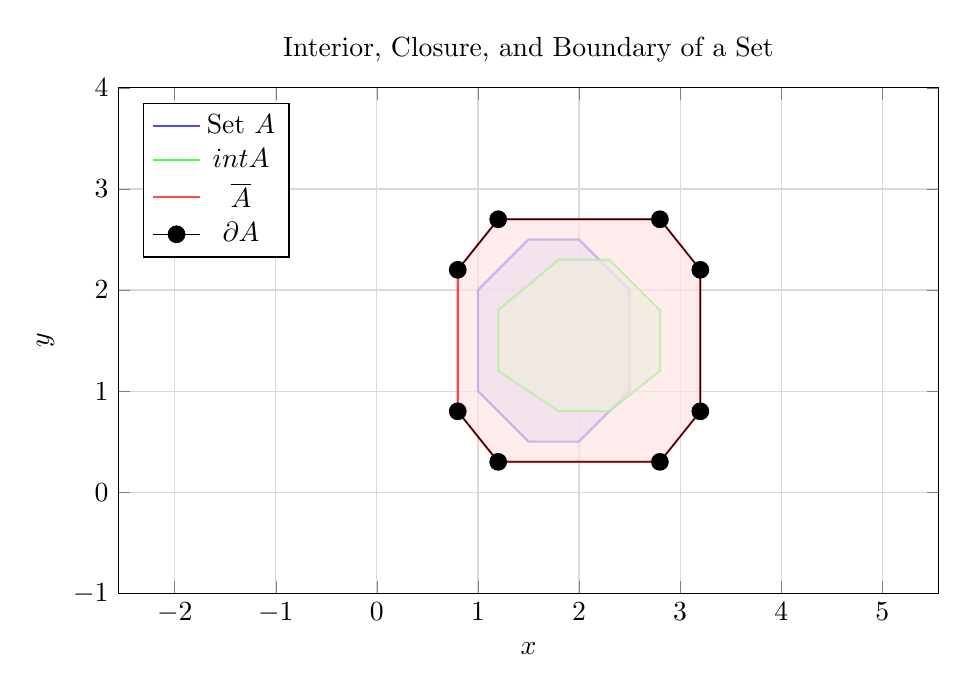
\begin{tikzpicture}
\begin{axis}[
    width=12cm,
    height=8cm,
    xlabel={$x$},
    ylabel={$y$},
    title={Interior, Closure, and Boundary of a Set},
    xmin=-1, xmax=4,
    ymin=-1, ymax=4,
    grid=major,
    grid style={gray!30},
    legend pos=north west,
    axis equal
]

% Original set A (open disk with some boundary points)
\addplot[blue, thick, fill=blue!20, opacity=0.7] coordinates {
    (1,1) (1.5,0.5) (2,0.5) (2.5,1) (2.5,2) (2,2.5) (1.5,2.5) (1,2) (1,1)
};
\addlegendentry{Set $A$}

% Interior of A (smaller open disk)
\addplot[green, thick, fill=green!20, opacity=0.7] coordinates {
    (1.2,1.2) (1.8,0.8) (2.3,0.8) (2.8,1.2) (2.8,1.8) (2.3,2.3) (1.8,2.3) (1.2,1.8) (1.2,1.2)
};
\addlegendentry{$\text{int } A$}

% Closure of A (larger closed disk)
\addplot[red, thick, fill=red!10, opacity=0.7] coordinates {
    (0.8,0.8) (1.2,0.3) (2.8,0.3) (3.2,0.8) (3.2,2.2) (2.8,2.7) (1.2,2.7) (0.8,2.2) (0.8,0.8)
};
\addlegendentry{$\overline{A}$}

% Boundary points
\addplot[black, mark=*, mark size=3pt] coordinates {
    (0.8,0.8) (1.2,0.3) (2.8,0.3) (3.2,0.8) (3.2,2.2) (2.8,2.7) (1.2,2.7) (0.8,2.2)
};
\addlegendentry{$\partial A$}

\end{axis}
\end{tikzpicture}
\caption{Relationships between interior, closure, and boundary: $\text{int } A \subseteq A \subseteq \overline{A}$ and $\partial A = \overline{A} \setminus \text{int } A$.}
\end{figure}

\bigskip\noindent\textbf{Solution:} Let $x \in \text{int } A$. Then there exists $\varepsilon > 0$ such that $B(x;\varepsilon) \subset A$. This means $B(x;\varepsilon) \cap (M - A) = \emptyset$, so $x \notin \overline{M - A}$. Therefore, $x \in M - \overline{M - A}$.

Conversely, let $x \in M - \overline{M - A}$. Then $x \notin \overline{M - A}$, so there exists $\varepsilon > 0$ such that $B(x;\varepsilon) \cap (M - A) = \emptyset$. This means $B(x;\varepsilon) \subset A$, so $x \in \text{int } A$.\qed


\begin{problembox}[3.44: Interior of Complement]
\begin{problemstatement}
Prove that \(\text{int }(M - A) = M - \overline{A}\).
\end{problemstatement}
\end{problembox}

\noindent\textbf{Strategy:} Use the same approach as Exercise 3.43 but with the roles of $A$ and $M-A$ reversed. Show that a point is interior to the complement if and only if it's not in the closure of $A$.

\bigskip\noindent\textbf{Solution:} Let $x \in \text{int }(M - A)$. Then there exists $\varepsilon > 0$ such that $B(x;\varepsilon) \subset M - A$. This means $B(x;\varepsilon) \cap A = \emptyset$, so $x \notin \overline{A}$. Therefore, $x \in M - \overline{A}$.

Conversely, let $x \in M - \overline{A}$. Then $x \notin \overline{A}$, so there exists $\varepsilon > 0$ such that $B(x;\varepsilon) \cap A = \emptyset$. This means $B(x;\varepsilon) \subset M - A$, so $x \in \text{int }(M - A)$.\qed


\begin{problembox}[3.45: Idempotence of Interior]
\begin{problemstatement}
Prove that \(\text{int }(\text{int } A) = \text{int } A\).
\end{problemstatement}
\end{problembox}

\noindent\textbf{Strategy:} Show both inclusions. The forward inclusion is clear since the interior of a subset is contained in the subset. For the reverse inclusion, use the fact that if a point is interior to $A$, it has a neighborhood in $A$, and since that neighborhood is open, it's contained in the interior of $A$.

\bigskip\noindent\textbf{Solution:} Since $\text{int } A \subseteq A$, we have $\text{int }(\text{int } A) \subseteq \text{int } A$.

For the reverse inclusion, let $x \in \text{int } A$. Then there exists $\varepsilon > 0$ such that $B(x;\varepsilon) \subset A$. Since $B(x;\varepsilon)$ is open and contained in $A$, we have $B(x;\varepsilon) \subset \text{int } A$. Therefore, $x \in \text{int }(\text{int } A)$.\qed


\begin{problembox}[3.46: Interior of Intersections]
\begin{problemstatement}
\begin{enumerate}[label=\alph*)]
\item Prove that \(\text{int } \left(\bigcap_{i=1}^n A_i\right) = \bigcap_{i=1}^n (\text{int } A_i)\), where each \( A_i \subseteq M \).
\item Show that \(\text{int } \left(\bigcap_{A \in F} A\right) \subseteq \bigcap_{A \in F} (\text{int } A)\) if \( F \) is an infinite collection of subsets of \( M \).
\item Give an example where equality does not hold in (b).
\end{enumerate}
\end{problemstatement}
\end{problembox}

\noindent\textbf{Strategy:} For (a), show both inclusions using the fact that if a point is interior to the intersection, it has a neighborhood in each set. For (b), show the inclusion using the same logic. For (c), use nested intervals that shrink to a single point.

\bigskip\noindent\textbf{Solution:} 
(a) Let $x \in \text{int }(\bigcap_{i=1}^n A_i)$. Then there exists $\varepsilon > 0$ such that $B(x;\varepsilon) \subset \bigcap_{i=1}^n A_i$. This means $B(x;\varepsilon) \subset A_i$ for each $i$, so $x \in \text{int } A_i$ for each $i$. Therefore, $x \in \bigcap_{i=1}^n (\text{int } A_i)$.

Conversely, let $x \in \bigcap_{i=1}^n (\text{int } A_i)$. Then for each $i$, there exists $\varepsilon_i > 0$ such that $B(x;\varepsilon_i) \subset A_i$. Let $\varepsilon = \min\{\varepsilon_1, \ldots, \varepsilon_n\}$. Then $B(x;\varepsilon) \subset \bigcap_{i=1}^n A_i$, so $x \in \text{int }(\bigcap_{i=1}^n A_i)$.

(b) Let $x \in \text{int }(\bigcap_{A \in F} A)$. Then there exists $\varepsilon > 0$ such that $B(x;\varepsilon) \subset \bigcap_{A \in F} A$. This means $B(x;\varepsilon) \subset A$ for each $A \in F$, so $x \in \text{int } A$ for each $A \in F$. Therefore, $x \in \bigcap_{A \in F} (\text{int } A)$.

(c) Let $F = \{A_n : n \in \mathbb{N}\}$ where $A_n = (-1/n, 1/n)$. Then $\bigcap_{A \in F} A = \{0\}$, so $\text{int }(\bigcap_{A \in F} A) = \emptyset$. However, $\text{int } A_n = A_n$ for each $n$, so $\bigcap_{A \in F} (\text{int } A) = \bigcap_{n=1}^{\infty} A_n = \{0\}$.\qed


\begin{problembox}[3.47: Interior of Unions]
\begin{problemstatement}
\begin{enumerate}[label=\alph*)]
\item Prove that \(\bigcup_{A \in F} (\text{int } A) \subseteq \text{int } \left(\bigcup_{A \in F} A\right)\).
\item Give an example of a finite collection \( F \) in which equality does not hold in (a).
\end{enumerate}
\end{problemstatement}
\end{problembox}

\noindent\textbf{Strategy:} For (a), show that if a point is interior to any set in the collection, it's interior to the union. For (b), use closed intervals that share a boundary point, where the union has interior points not in the union of interiors.

\bigskip\noindent\textbf{Solution:} 
(a) Let $x \in \bigcup_{A \in F} (\text{int } A)$. Then $x \in \text{int } A$ for some $A \in F$. There exists $\varepsilon > 0$ such that $B(x;\varepsilon) \subset A \subset \bigcup_{A \in F} A$. Therefore, $x \in \text{int }(\bigcup_{A \in F} A)$.

(b) Let $F = \{A, B\}$ where $A = [0,1]$ and $B = [1,2]$. Then $\text{int } A = (0,1)$ and $\text{int } B = (1,2)$, so $\bigcup_{A \in F} (\text{int } A) = (0,1) \cup (1,2)$. However, $\bigcup_{A \in F} A = [0,2]$, so $\text{int }(\bigcup_{A \in F} A) = (0,2)$, which properly contains $(0,1) \cup (1,2)$.\qed


\begin{problembox}[3.48: Interior of Boundary]
\begin{problemstatement}
\begin{enumerate}[label=\alph*)]
\item Prove that \(\text{int } (\partial A) = \emptyset\) if \( A \) is open or if \( A \) is closed in \( M \).
\item Give an example in which \(\text{int } (\partial A) = M\).
\end{enumerate}
\end{problemstatement}
\end{problembox}

\noindent\textbf{Strategy:} For (a), use the fact that the boundary of an open set is the closure minus the interior, and for a closed set it's the set minus the interior. In both cases, the boundary contains no open balls. For (b), use the rationals in $\mathbb{R}$ where the boundary is all of $\mathbb{R}$.

\bigskip\noindent\textbf{Solution:} 
(a) If $A$ is open, then $\partial A = \overline{A} \setminus \text{int } A = \overline{A} \setminus A$. If $A$ is closed, then $\partial A = A \setminus \text{int } A$.

In both cases, $\partial A$ contains no open balls, so $\text{int } (\partial A) = \emptyset$.

(b) Let $A = \mathbb{Q}$ in the metric space $\mathbb{R}$. Then $\partial A = \mathbb{R}$, so $\text{int } (\partial A) = \mathbb{R} = M$.\qed


\begin{problembox}[3.49: Interior of Union of Sets with Empty Interior]
\begin{problemstatement}
If \(\text{int } A = \text{int } B = \emptyset\) and if \(A\) is closed in \(M\), then \(\text{int } (A \cup B) = \emptyset\).
\end{problemstatement}
\end{problembox}

\noindent\textbf{Strategy:} Use the fact that if a closed set has empty interior, every point is a limit point. Show that any point in the union cannot have a neighborhood entirely contained in the union by using the properties of limit points and the fact that $B$ has empty interior.

\bigskip\noindent\textbf{Solution:} Since $A$ is closed, $\text{int } A = \emptyset$ implies that $A$ has no isolated points. Therefore, every point in $A$ is a limit point of $A$.

Let $x \in A \cup B$. If $x \in A$, then every neighborhood of $x$ contains points of $A$ different from $x$. Since $A \subset A \cup B$, every neighborhood of $x$ contains points of $A \cup B$ different from $x$, so $x$ is not an interior point of $A \cup B$.

If $x \in B \setminus A$, then since $\text{int } B = \emptyset$, every neighborhood of $x$ contains points not in $B$. Since $A$ is closed and $x \notin A$, there exists a neighborhood of $x$ that doesn't intersect $A$. This neighborhood contains points not in $A \cup B$, so $x$ is not an interior point of $A \cup B$.

Therefore, $\text{int } (A \cup B) = \emptyset$.\qed


\begin{problembox}[3.50: Counterexample for Union of Sets with Empty Interior]
\begin{problemstatement}
Give an example in which \(\text{int } A = \text{int } B = \emptyset\) but \(\text{int } (A \cup B) = M\).
\end{problemstatement}
\end{problembox}

\noindent\textbf{Strategy:} Use the rational and irrational numbers in $\mathbb{R}$. Both have empty interior (since they're dense and co-dense), but their union is all of $\mathbb{R}$ which has non-empty interior.

\bigskip\noindent\textbf{Solution:} Let $A = \mathbb{Q}$ and $B = \mathbb{R} \setminus \mathbb{Q}$ in the metric space $\mathbb{R}$. Then $\text{int } A = \emptyset$ and $\text{int } B = \emptyset$, but $A \cup B = \mathbb{R}$, so $\text{int } (A \cup B) = \mathbb{R} = M$.



\begin{problembox}[3.51: Properties of Boundary]
\begin{problemstatement}
Prove that:
\[
\partial A = \overline{A} \cap \overline{M - A} \quad \text{and} \quad \partial A = \partial(M - A).
\]
\end{problemstatement}
\end{problembox}

\noindent\textbf{Strategy:} For the first equality, use the definition of boundary as points that are adherent to both the set and its complement. For the second equality, use the first equality and the fact that the complement of the complement is the original set.

\bigskip\noindent\textbf{Solution:} For the first equality, $x \in \partial A$ if and only if every neighborhood of $x$ contains both points of $A$ and points of $M - A$. This means $x \in \overline{A}$ and $x \in \overline{M - A}$, so $x \in \overline{A} \cap \overline{M - A}$.

For the second equality, $\partial A = \overline{A} \cap \overline{M - A} = \overline{M - A} \cap \overline{A} = \partial(M - A)$.\qed


\begin{problembox}[3.52: Boundary of Union under Disjoint Closures]
\begin{problemstatement}
If \(\overline{A} \cap \overline{B} = \emptyset\), then \(\partial(A \cup B) = \partial A \cup \partial B\).
\end{problemstatement}
\end{problembox}

\noindent\textbf{Strategy:} Use the fact that when closures are disjoint, the closure of the union is the union of closures. Show both inclusions by using the definition of boundary and the disjointness condition to separate the contributions from $A$ and $B$.

\bigskip\noindent\textbf{Solution:} Since $\overline{A} \cap \overline{B} = \emptyset$, we have $\overline{A \cup B} = \overline{A} \cup \overline{B}$.

Let $x \in \partial(A \cup B)$. Then $x \in \overline{A \cup B} = \overline{A} \cup \overline{B}$ and $x \in \overline{M - (A \cup B)} = \overline{(M - A) \cap (M - B)} \subseteq \overline{M - A} \cap \overline{M - B}$.

If $x \in \overline{A}$, then $x \in \overline{A} \cap \overline{M - A} = \partial A$. If $x \in \overline{B}$, then $x \in \overline{B} \cap \overline{M - B} = \partial B$. Therefore, $x \in \partial A \cup \partial B$.

Conversely, let $x \in \partial A \cup \partial B$. Without loss of generality, assume $x \in \partial A$. Then $x \in \overline{A} \subseteq \overline{A \cup B}$ and $x \in \overline{M - A} \subseteq \overline{M - (A \cup B)}$. Therefore, $x \in \partial(A \cup B)$.


\section{Solving and Proving Techniques}

\subsection*{Proving Sets are Open}
\begin{itemize}
\item Use the definition: show every point has a neighborhood contained in the set
\item Use the fact that unions of open sets are open
\item Use the fact that finite intersections of open sets are open
\item Use the fact that open balls are open sets
\item Use the fact that products of open intervals are open
\item Use the fact that the interior of any set is open
\end{itemize}

\subsection*{Proving Sets are Closed}
\begin{itemize}
\item Show the complement is open
\item Use the fact that intersections of closed sets are closed
\item Use the fact that finite unions of closed sets are closed
\item Use the fact that the closure of any set is closed
\item Use the fact that finite sets are closed
\item Use the fact that closed balls are closed sets
\end{itemize}

\subsection*{Finding Accumulation Points}
\begin{itemize}
\item Look for points that can be approached by sequences in the set
\item Use density properties (rationals, irrationals are dense in $\mathbb{R}$)
\item Consider convergence of sequences to boundary points
\item Use the fact that accumulation points of accumulation points are accumulation points
\item Use the fact that accumulation points of unions are unions of accumulation points
\item Consider geometric intuition for sets in $\mathbb{R}^2$ and $\mathbb{R}^3$
\end{itemize}

\subsection*{Working with Interior and Closure}
\begin{itemize}
\item Use the definition: interior points have neighborhoods in the set
\item Use the fact that interior is the largest open subset
\item Use the fact that closure is the smallest closed superset
\item Use the relationship: $\text{int } A = M - \overline{M - A}$
\item Use the relationship: $\overline{A} = A \cup A'$ where $A'$ is the derived set
\item Use the fact that interior of interior equals interior
\item Use the fact that closure of closure equals closure
\end{itemize}

\subsection*{Proving Countability}
\begin{itemize}
\item Use the fact that countable unions of countable sets are countable
\item Use the fact that Cartesian products of countable sets are countable
\item Use the fact that subsets of countable sets are countable
\item Use the fact that images of countable sets under injective functions are countable
\item Use the Lindelöf property in separable spaces
\item Use the fact that isolated points form a countable set
\item Use the fact that disjoint open sets in separable spaces are countable
\end{itemize}

\subsection*{Working with Compactness}
\begin{itemize}
\item Use the Heine-Borel theorem: closed and bounded in $\mathbb{R}^n$
\item Use the fact that closed subsets of compact sets are compact
\item Use the fact that finite unions of compact sets are compact
\item Use the fact that intersections of compact sets are compact
\item Use the fact that continuous images of compact sets are compact
\item Use the fact that compactness is independent of the ambient space
\item Use the fact that compact sets are closed and bounded
\end{itemize}

\subsection*{Using Density Properties}
\begin{itemize}
\item Use the fact that rationals and irrationals are dense in $\mathbb{R}$
\item Use the fact that $\mathbb{Q}^n$ is dense in $\mathbb{R}^n$
\item Use the fact that dense sets intersect every open set
\item Use the fact that if $A$ is dense in $S$ and $S$ is dense in $T$, then $A$ is dense in $T$
\item Use the fact that dense sets in open sets are dense in the whole space
\item Use the fact that intersections of dense and open sets are dense
\end{itemize}

\subsection*{Working with Metric Spaces}
\begin{itemize}
\item Use the triangle inequality to bound distances
\item Use the fact that metric balls are open sets
\item Use the fact that closed balls are closed sets
\item Use the fact that finite sets are closed
\item Use the fact that separable spaces have the Lindelöf property
\item Use the fact that bounded metrics can be constructed from unbounded ones
\item Use the fact that product metrics satisfy the metric axioms
\end{itemize}

\subsection*{Proving Connectedness}
\begin{itemize}
\item Use proof by contradiction: assume the space can be split into two non-empty disjoint open sets
\item Use the fact that $\mathbb{R}^1$ and $\mathbb{R}^n$ are connected
\item Use the fact that connected spaces cannot have non-trivial clopen subsets
\item Use the fact that continuous images of connected sets are connected
\item Use the fact that unions of connected sets with non-empty intersection are connected
\end{itemize}

\subsection*{Using Proof by Contradiction}
\begin{itemize}
\item Assume the opposite of what you want to prove
\item Use the properties of open and closed sets to derive a contradiction
\item Use the fact that limits must be unique
\item Use the fact that countable sets cannot be uncountable
\item Use the fact that compact sets must have finite subcovers
\item Use the fact that connected spaces cannot be split into disjoint open sets
\item Use the Cantor intersection theorem to find contradictions
\end{itemize}

\subsection*{Working with Sequences}
\begin{itemize}
\item Use the fact that convergent sequences have unique limits
\item Use the fact that subsequences of convergent sequences converge to the same limit
\item Use the fact that bounded sequences have convergent subsequences
\item Use the fact that Cauchy sequences converge in complete spaces
\item Use the fact that accumulation points can be approached by sequences
\item Use the fact that closed sets contain limits of convergent sequences
\end{itemize}

\subsection*{Proving Uniqueness}
\begin{itemize}
\item Use the fact that closures are unique
\item Use the fact that interiors are unique
\item Use the fact that accumulation points are well-defined
\item Use the fact that limits of sequences are unique
\item Use the fact that compact sets have unique properties
\item Use the fact that dense subsets are unique up to closure
\end{itemize}

\subsection*{Working with Boundaries}
\begin{itemize}
\item Use the definition: $\partial A = \overline{A} \cap \overline{M - A}$
\item Use the fact that boundaries of complements are the same
\item Use the fact that boundaries of unions can be related to boundaries of components
\item Use the fact that boundaries of open or closed sets have empty interior
\item Use the fact that boundaries are closed sets
\item Use the fact that boundaries separate sets from their complements
\end{itemize}

